\chapter{Controlador de corriente} \chapterlabel{Informe/4-ControladorCorriente} \label{cap:ControladorCorriente}
\colorbox{red}{no nos olvidemos de actualizar esto cuando terminemos}
En este capítulo se diseña y modela el circuito encargado de controlar la corriente que circula por el electroimán. Como se vio en el capítulo anterior, el sistema trabaja con corrientes elevadas por lo que se implementan estrategias de conmutación para reducir las pérdidas de energía. Para ello se utiliza una topología de puente H con cuatro MOSFET y un \textsl{driver} que los controla. Además, se detallan los criterios tenidos en cuenta al momento de  elegir  y dimensionar todos los componentes que intervienen para lograr el correcto funcionamiento del controlador de corriente. Por último, se obtiene su función transferencia  para ser utilizada en el diseño del compensador.

\section{Descripción general}\label{sec_descripcion-general}

Para controlar la posición de la pieza móvil es necesario modificar la fuerza que ejerce el electroimán sobre ella. Como se analizó en el capítulo \ref{cap:CaracterizacionElectroiman}, dicha fuerza está determinada por la ecuación \ref{eq_fuerza_magnetica}, que se repite a continuación. 

\begin{equation*}
	\abs{F_{m}}=\frac{i^{2}*N^{2}*\mu_{o}*A}{4*Y_{g}^{2}}
\end{equation*}

En ella se ve que la fuerza magnética depende de la corriente del bobinado. Por lo tanto, se propone implementar un controlador que permita regular la corriente a partir de una tensión de entrada, que funciona como referencia del valor de corriente deseado. De forma tal que, al variar dicha tensión, se logre ajustar la corriente y, por ende, la fuerza ejercida por el electroimán.

%En ella se ve que la fuerza magnética depende de la corriente del bobinado. Por lo tanto, se propone implementar un controlador de corriente que permita regularla. Este controlador tendrá como entrada una tensión de referencia correspondiente al valor de corriente deseado. De esta forma, al variar dicha tensión, se logra ajustar la fuerza ejercida por el electroimán.

\subsection{Comportamiento eléctrico del electroimán}\label{sec_comportamiento-electrico-electroiman}

Como se analizó en el capítulo \ref{cap:CaracterizacionElectroiman}, el electroimán puede ser modelado como una inductancia que varía con la distancia de entrehierro ($L(Y_g)$) y una resistencia serie ($R_L$). Es decir, como un circuito RL serie cuya admitancia, o relación entre corriente de salida ($I_L$) y tensión de entrada ($V_L$), es:

\begin{equation} \label{eq_corriente}
	\frac{I_L}{V_L}(s)=\frac{1}{s*L(Y_g)+R_L}
\end{equation}

Al aplicar la transformada inversa de Laplace a la expresión  \ref{eq_corriente}, se obtiene la respuesta temporal de la corriente ante un escalón de tensión en la entrada con amplitud $v_L$, considerando corriente inicial $I_o$ y constante de tiempo $\tau=\frac{L(Y_g)}{R_L}$.

\begin{equation} \label{eq_corriente_temporal_cond_iniciales}
	i_L(t)=\frac{v_L}{R_L} + (I_o-\frac{v_L}{R_L})*e^{-\frac{t}{\tau}}
\end{equation}

En la expresión \ref{eq_corriente_temporal_cond_iniciales} se puede observar que la respuesta al escalón está compuesta por dos partes: un término con una exponencial negativa correspondiente al transitorio, y un término constante correspondiente al valor en régimen permanente $\frac{v_L}{R_L}$. El primero es el responsable de que la corriente en el inductor crezca de manera amortiguada, hasta alcanzar el valor de régimen permanente luego de cierto tiempo. Este comportamiento se puede observar en la simulación realizada en la figura \ref{fig:img_respuesta_escalon}. En la parte superior se observa la tensión de entrada y, en la inferior, la corriente del electroimán. Este análisis resulta de utilidad para conocer el comportamiento del electroimán y diseñar un controlador de corriente adecuado.


\begin{figure}[H]
	\centering
	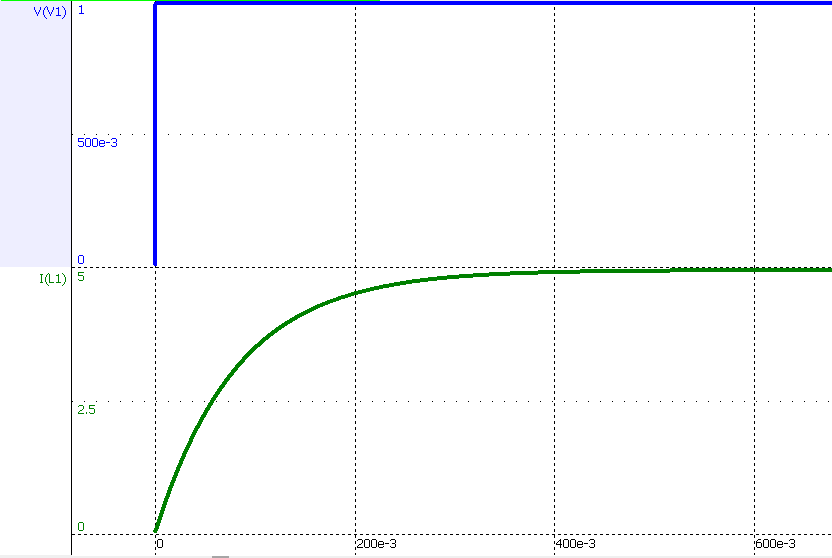
\includegraphics[scale=0.5]{corriente_escalon.png}
	\caption{Respuesta ante una entrada en escalón.}
	\label{fig:img_respuesta_escalon}
\end{figure}

\colorbox{red}{ver si se puede mejorar esta imagen..}

\section{Diseño del controlador}

Se desea controlar el valor de la corriente que circula por el electroimán a partir de una tensión de referencia. Es decir, que la corriente ($I_L$) sea proporcional a esta tensión de entrada ($V_{IL_{ref}}$). Para ello, se propone implementar un controlador que actúe sobre la tensión de alimentación del electroimán ($V_L$), ya que como se ve en la expresión \ref{eq_corriente}, esta permite modificar el valor de la corriente. En la figura \ref{fig:img_diagrama_bloques_basico_cc} se ilustra el diagrama en bloques propuesto para el controlador.

%\begin{figure}[H]
%	\centering
%	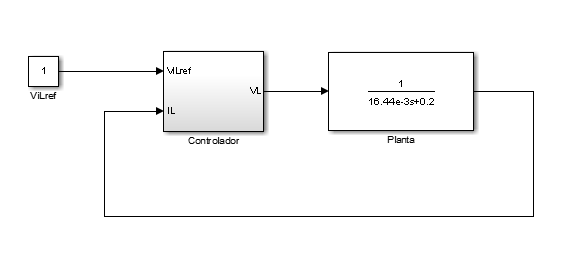
\includegraphics[scale=0.5]{Diagrama-en-bloques-basico.png}
%	\caption{Diagrama en bloques básico.}
%	\label{fig:img_diagrama_bloques_basico_cc}
%\end{figure}

\begin{figure}[H]
	\centering
	%Acá se define eñ diagrama en bloques completo
\begin{tikzpicture}[auto, node distance=3cm,>=latex']
	% We start by placing the blocks
	\node [input, name=input] {};
	\node [block, right of=input] (controller) {CONTROLADOR};
	\node [block, right of=controller, 
	node distance=4.5cm] (system) {${\displaystyle\frac{1}{s*L(Y_g)+R_L}}$};
	% We draw an edge between the controller and system block to 
	% calculate the coordinate u. We need it to place the measurement block. 
	\draw [->] (controller) -- node[name=u] {$V_L$} (system);
	\node [output, right of=system] (output) {};
	\node [coordinate, below of=u] (measurements) {Measurements};
	
	% Once the nodes are placed, connecting them is easy. 
	\draw [draw,->] (input) -- node[pos=0.5]{$V_{IL_{ref}}$} (controller);
	\draw [->] (system) -- node [name=y] {$I_L$}(output);
	\draw  (y) |- (measurements);
	\draw [->] (measurements) -| node[pos=0.9]{$I_L$} (controller); %node [near end] {$I_{L_{feed}}$} 
\end{tikzpicture}


	
	\caption{Diagrama en bloques del controlador de corriente.}
	\label{fig:img_diagrama_bloques_basico_cc}
\end{figure}

Este sistema de control trabaja a lazo cerrado, es decir, mide una tensión proporcional a la corriente y luego la compara con la referencia. Este resultado es utilizado para determinar si es necesario aumentar o disminuir la corriente y, en función de ello, actuar sobre la tensión de alimentación del electroimán.

Para controlar la tensión de alimentación del electroimán se propone diseñar un controlador que trabaje en conmutación. En este tipo de controladores se alterna la alimentación del electroimán ($V_L$) entre un valor superior positivo $\ V_{sup}$, y un valor inferior negativo $V_{inf}$. De esta manera, al controlar los tiempos de conmutación, se logra que la corriente oscile en torno a un valor medio deseado y se obtiene una forma de onda como la que se muestra en la figura  \ref{fig:img_corriente_exponencial}. En ella se puede ver que esta manera de controlar la alimentación genera una corriente con oscilaciones alrededor del valor medio deseado, también conocidas como \textsl{ripple}. Sin embargo, esto no presentaría un problema si el controlador de corriente es diseñado de forma tal que estas variaciones sean pequeñas comparadas con el valor medio ya que no afectarían en la fuerza ejercida.

\begin{figure}[H]
	\centering
	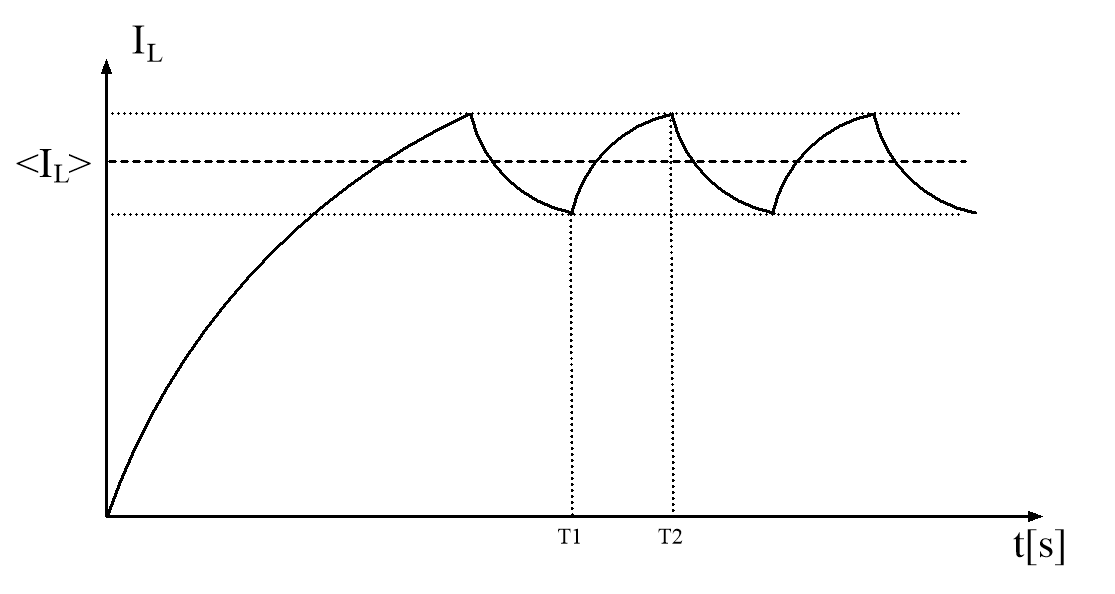
\includegraphics[scale=0.5]{Forma-de-onda-corriente-exponencial.png}
	\caption{Forma de onda de corriente y tensión en el electroimán.}
	\label{fig:img_corriente_exponencial}
\end{figure}

Al elegir un período de conmutación lo suficientemente pequeño con respecto a la constante de tiempo de la planta, la forma de onda de la corriente en estado estacionario puede ser aproximada a una onda triangular como se muestra en la figura \ref{fig:img_corriente_lineal}. 

\begin{figure}[H]
	\centering
	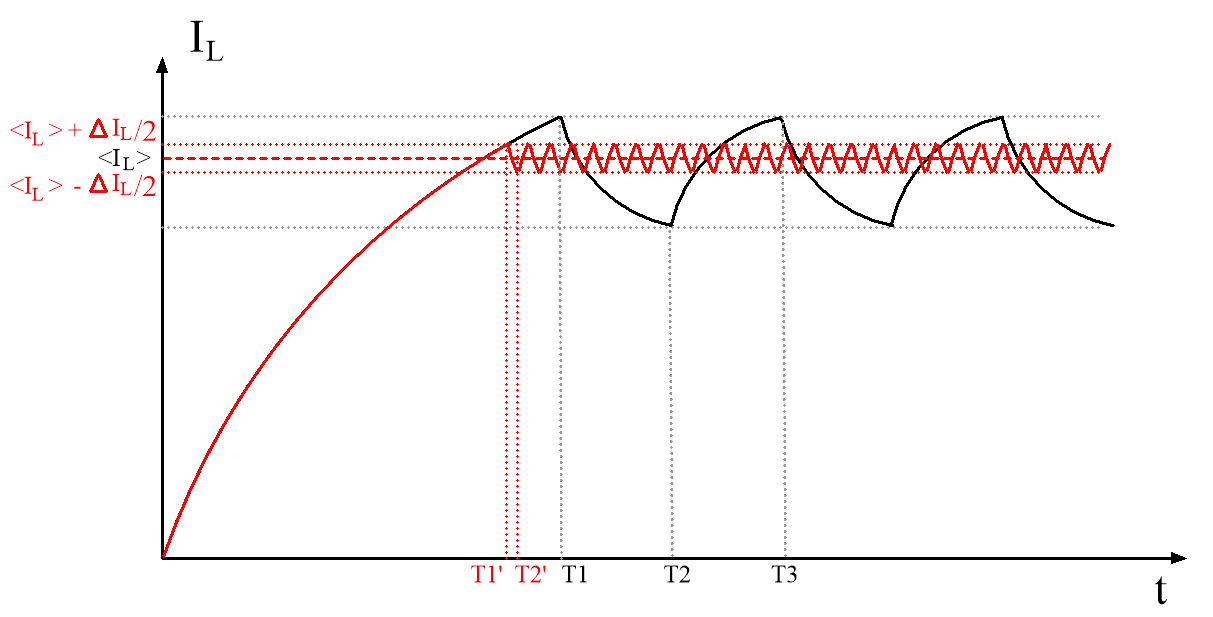
\includegraphics[scale=0.5]{Forma-de-onda-corriente-lineal.png}
	\caption{Forma de onda de corriente al disminuir el período de conmutación.}
	\label{fig:img_corriente_lineal}
\end{figure}

Cada tramo que compone la onda triangular puede ser aproximado con la ecuación \ref{eq_corriente_taylor}, en donde $I_o$ corresponde al valor de corriente en el instante en que se produce la conmutación en $V_L$.

\begin{equation} \label{eq_corriente_taylor}
	i_L(t)=I_o -  (I_o-\frac{V_L}{R_L})*\frac{t}{\tau}
\end{equation}

Es posible observar en la expresión \ref{eq_corriente_taylor} que la pendiente de la onda triangular depende de $\tau=\frac{L_{(Y_g)}}{R_L}$. Es decir, existe una relación entre la pendiente y la distancia de entrehierro. Como se mencionó en la sección \ref{sec_descripcion-del-dispositivo}, para que el dispositivo de levitación magnética pueda mantener la pieza móvil suspendida debe conocer dicha distancia en todo momento. Por lo tanto se propone medirla indirectamente a través de la pendiente de la onda triangular. A continuación se analizará qué variables del sistema afectan el valor de la pendiente y si es posible utilizarla para estimar la posición.

\subsection{Análisis de estimación de distancia de entrehierro} \label{sec_analisis_estimacion}

Como se mencionó previamente, la pendiente de la onda triangular de la corriente contiene información de la distancia de entrehierro. Por lo tanto, se propone estimar el valor de la distancia a partir de la medición de dicha pendiente. 

Para comenzar este análisis se deriva la expresión \ref{eq_corriente_taylor} con respecto al tiempo para obtener el valor de la pendiente y se reemplaza $\tau=\frac{L(Y_g)}{R_L}$:

%\begin{equation} \label{eq_derivada_corriente}
%	\frac{di_L(t)}{dt}=(\frac{V_L}{R_L}-I_o)*\frac{1}{\tau}
%\end{equation}

\begin{equation} \label{eq_derivada_corriente}
	\frac{di_L(t)}{dt}=\frac{V_L-I_o*R_L}{L(Y_g)}
\end{equation}

Si bien la pendiente cambia según las condiciones iniciales, para este análisis se considera $I_o=0$ y luego se analizará cómo afecta esta suposición en el sistema real. De esta forma, la pendiente resulta:
\colorbox{red}{No nos olvidemos de verificar esta suposición...}


\begin{equation} \label{eq_derivada_corriente_2}
	\frac{di_L(t)}{dt}= \frac{V_L}{L(Y_g)}
\end{equation}


Como se vio en el capítulo \ref{cap:CaracterizacionElectroiman}, la expresión \ref{eq_inductancia_vs_y} indica que la inductancia del electroimán es inversamente proporcional a la distancia de entrehierro. Por lo tanto, reemplazando $L(Y_g)$ en la ecuación \ref{eq_derivada_corriente_2} se llega a:

\begin{equation}\label{eq_pendiente_vs_Yg}
	\frac{di_L(t)}{dt}= Y_g*\frac{2}{N^2*A*\mu_o}*V_L
\end{equation}

En la expresión \ref{eq_pendiente_vs_Yg}, la tensión con la que se alimenta al electroimán está representada por $V_L$. A partir de la figura \ref{fig:img_corriente_lineal} se pueden plantear dos casos para la pendiente: cuando crece (con $V_L=V_{sup}$) y cuando decrece (con $V_L=V_{inf}$). Por lo tanto, se obtienen dos expresiones:

\begin{equation} 
	\frac{di_L(t)}{dt}_{sup}= Y_g*\frac{2}{N^2*A*\mu_o}*V_{sup}
\end{equation}


\begin{equation}
	\frac{di_L(t)}{dt}_{inf}= Y_g*\frac{2}{N^2*A*\mu_o}*V_{inf}
\end{equation}
%
%La tensión $V_L$ es un parámetro de diseño en el sistema, por lo tanto resulta conveniente elegir una fuente de alimentación para el electroimán que sea capaz de entregar una tensión, que llamaremos $V_{cc}$, alternando su polaridad. Por lo tanto $|V_{sup}|=|V_{inf}|=|V_{cc}|$. De esta forma, se obtiene que el módulo de la pendiente es igual en ambos casos y resulta:
%
%La tensión $V_L$ es un parámetro de diseño en el sistema, por lo tanto resulta conveniente elegir una alimentación $V_{cc}$ tal que $|V_{sup}|=|V_{inf}|=|V_{cc}|$. De esta forma, se obtiene que el módulo de la pendiente es igual en ambos casos y resulta:

Como se desea realizar la estimación a partir del módulo de la pendiente, resulta conveniente que su magnitud sea igual en cada ciclo de conmutación independientemente de la tensión de alimentación aplicada. Por lo tanto, debido a que la tensión $V_L$ es un parámetro de diseño en el sistema, se eligen valores de $V_{sup}$ y $V_{inf}$ que difieran en su polaridad, pero que tengan la misma magnitud. De esta forma, se define un valor para la tensión de alimentación $V_{cc}$ tal que $|V_{sup}|=|V_{inf}|=|V_{cc}|$ y se obtiene:
 
\begin{equation} \label{eq_pendiente_simetrica_corriente}
	\abs{\frac{di_L(t)}{dt}}= Y_g*\frac{2}{N^2*A*\mu_o}*\abs{V_{cc}}
\end{equation}

Como se muestra en la ecuación \ref{eq_pendiente_simetrica_corriente}, la pendiente varía únicamente con la distancia $Y_g$ puesto que los demás términos son constantes. 

De este análisis se llega a la conclusión de que es posible obtener una estimación de la distancia de entrehierro a partir de la medición de la pendiente de la onda triangular. Para ello se debe diseñar una fuente de alimentación que permita alternar la polaridad de la tensión aplicada al electroimán con igual magnitud pero sentido contrario.

\subsection{Lógica de control de corriente}

Para controlar la corriente que circula por el electroimán y lograr la forma de onda triangular, se propone un controlador del tipo ON-OFF con el agregado de una zona de histéresis.

En la figura \ref{fig:img_diag-en-bloques} se puede observar el controlador implementado, en el cual la diferencia entre la corriente de referencia y la que circula por el electroimán está representada por $e$. Esta última ingresa a un comparador con histéresis, que se encarga de alternar la polaridad de la tensión del electroimán según el valor de $e$.

%\begin{figure}[H]
%	\centering
%	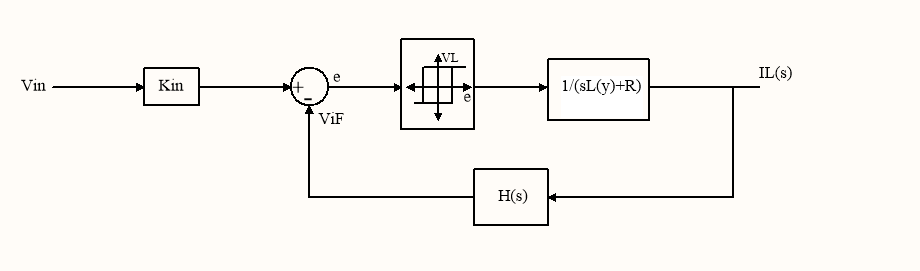
\includegraphics[width=\textwidth]{Diagrama-en-bloques.png}
%	\caption{Diagrama en bloques del controlador de corriente con histéresis.}
%	\label{fig:img_diag-en-bloques}
%\end{figure}

\begin{figure}[H]
	\centering
	%\begin{tikzpicture}[auto, node distance=2cm,>=latex']
%	\node [coordinate, name=entrada] {};
%	\node [sum, right=of entrada] (resta) {};
%	\node [coordinate, right=of resta] (ie) {};
%	\node [block, right=of ie] (comparador) {COMP};
%	\node [block, right=of comparador] (planta) {PLANTA};
%	\node [coordinate, right=of planta] (salida) {};
%	\node [coordinate, below of=planta] (realimentacion) {};
%	
%	\draw [->] (entrada) -- node {$I_{L_{ref}}$} (resta);
%	\draw [->] (resta) -- (comparador);
%	\draw [->] (comparador) -- (planta);
%%	\draw [->] (fft) -- node[name=a_resta] {} (resta);
%%	\draw [->] (fft) -- node[near end] {+} (resta);
%	\draw [->] (salida) |- (realimentacion);
%	\draw [->] (realimentacion) -| node[pos=0.95] {-} (resta);
%	\draw [->] (planta) -- node {$I_L$} (salida);
%	
%
%	
%%	\draw [->] (fft) |- (promedio);
%%	\draw [->] (promedio) -| node [near end] {-} (resta);
%\end{tikzpicture}

\tikzstyle{block} = [draw, fill=blue!20, rectangle, 
minimum height=3em, minimum width=6em]
\tikzstyle{sum} = [draw, fill=blue!20, circle, node distance=1cm]
\tikzstyle{input} = [coordinate]
\tikzstyle{output} = [coordinate]
\tikzstyle{pinstyle} = [pin edge={to-,thin,black}]

\def\windup{
	\tikz[remember picture,overlay]{
		\draw [stealth-stealth] (-1,0) -- node[pos=1] {$I_e$} (1,0); 
		\draw [stealth-stealth] (0,-0.6)--(0,0.6); %esto son los ejes
		\draw [-stealth] (-0.9,-0.4)-- (0.3,-0.4);
		\draw  [-stealth] (0.3,-0.4) -- (0.3,0.4); 
		\draw [-stealth] (0.9,0.4) --(-0.3,0.4);
		\draw [-stealth] (-0.3,0.4) -- (-0.3, -0.4); %esto sería la formita
}}
% The block diagram code is probably more verbose than necessary
\begin{tikzpicture}[auto, node distance=3cm,>=latex']
	% We start by placing the blocks
	\node [input, name=input] {};
	\node [sum, right of=input] (sum) {};
	\node [block, right of=sum] (controller) {\windup};
	\node [block, right of=controller, 
	node distance=3cm] (system) {System};
	% We draw an edge between the controller and system block to 
	% calculate the coordinate u. We need it to place the measurement block. 
	\draw [->] (controller) -- node[name=u] {$V_L$} (system);
	\node [output, right of=system] (output) {};
	\node [block, below of=u] (measurements) {Measurements};
	
	% Once the nodes are placed, connecting them is easy. 
	\draw [draw,->] (input) -- node {$I_{L_{ref}}$} (sum);
	\draw [->] (sum) -- node {$I_e$} (controller);
	\draw [->] (system) -- node [name=y] {$I_L$}(output);
	\draw [->] (y) |- (measurements);
	\draw [->] (measurements) -| node[pos=0.99] {$-$} 
	node [near end] {$I_{L_{feed}}$} (sum);
\end{tikzpicture}

	\caption{Diagrama en bloques simplificado del controlador de corriente}	\label{fig:img_diag-en-bloques}
\end{figure}

El controlador alterna la polaridad de la tensión de alimentación del electroimán, con el objetivo de que la corriente se mantenga oscilando en torno a un valor medio de referencia. Para ello se define un margen de corriente $\Delta I_L$ de forma tal que, si la corriente que circula por el electroimán supera a la de referencia, no se producirá un cambio de polaridad en la tensión aplicada hasta que la supere por $\frac{\Delta I_L}{2}$. Análogamente, cuando comienza a decrecer, seguirá haciéndolo hasta que sea menor a la corriente de referencia menos $\frac{\Delta I_L}{2}$.

Debido a que en las sucesivas conmutaciones lo único que cambia es la polaridad de la tensión con la que se excita al electroimán, la constante de tiempo del circuito no cambia. Esto da como resultado que la corriente oscile sobre un valor medio con igual tiempo de crecimiento que de decrecimiento. La amplitud de estas oscilaciones (o \textsl{ripple}) es fija y está determinada por el ancho de histéresis con el que se diseñe el controlador.

Para lograr una forma de onda como la mostrada en la  figura \ref{fig:img_corriente_lineal} el controlador debe actuar de la siguiente manera. Al iniciar, la corriente $I_L$ es cero, dando como resultado a la entrada del comparador  $e = I_{ref}$. Por lo tanto, el comparador excita al electroimán con $V_L=+V_{CC}$ provocando que $I_L$ aumente de forma exponencial hasta que el valor de $e$ sea $-\frac{\Delta I_L}{2}$. Una vez alcanzado este valor, el bloque con histéresis actúa y conmuta la tensión $V_L$ a $-V_{CC}$. Al hacer esto, la corriente comienza a decrecer hasta que el error sea igual a $\frac{\Delta I_L}{2}$. De igual forma, en este punto el bloque comparador actúa y la tensión $V_L$ conmuta a $+V_{CC}$. Este ciclo se repite indefinidamente siempre y cuando la $I_{ref}$ sea constante. En caso de que esta cambie, el sistema dejará de conmutar momentáneamente hasta que el módulo de $e$ sea igual a $\frac{\Delta I_L}{2}$. Una vez igualado, el sistema volverá a conmutar.

TENEMOS QUE PONER LA IMAGEN Y CAMBIAR EL TEXTO EN REFERENCIA A ELLA
\colorbox{red}{Que imagen sería?}

\subsection{Consideraciones prácticas del controlador de corriente}

En el diagrama en bloques \ref{fig:img_diag-en-bloques} se analizó la lógica de control trabajando únicamente con señales en forma de corriente. Sin embargo, para la realización práctica del controlador es conveniente trabajar con tensiones. Por lo tanto, es necesario  convertir el valor de corriente del electroimán medido en un valor de tensión proporcional. Esto se realiza utilizando un sensor de corriente cuya ganancia se simboliza con $H(s)$.

Para la señal de entrada $V_{IL_{ref}}$ se adoptan valores de tensión entre $0\:V$ y $5\:V$. Esto con el fin de que la implementación circuital utilice amplificadores operacionales con una fuente simple de $5\:V$. 

Por otro lado, para lograr que la corriente de salida excursione entre $0\:A$ a $30\:A$, a partir de una tensión de referencia de entrada ($V_{IL_{ref}}$), se agrega el bloque $K_{in}$. Este permite asociar cada valor de corriente de salida con uno de tensión de entrada.

En el bloque de histéresis del diagrama en bloques planteado hasta ahora, se mezclan señales de niveles lógicos en su entrada con señales de potencia en su salida. Para implementar el sistema de control real se deben separar estas etapas, de manera que el comparador con histéresis tenga una salida de tensión en niveles lógicos y luego haya un bloque que amplifique esta señal para ser utilizada como alimentación del electroimán.

En la figura \ref{fig:img_diag-en-bloques-conH-y-Kin} se muestra el diagrama en bloques del sistema teniendo en cuenta los aspectos previamente mencionados.

%\begin{figure}[H]
%	\centering
%	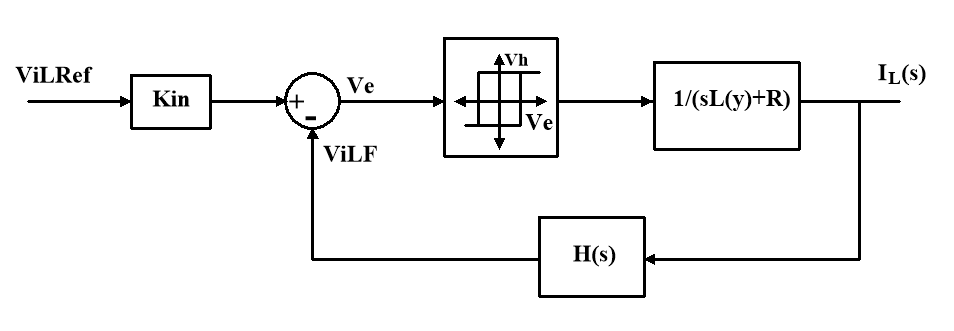
\includegraphics[width=\textwidth]{Diagrama-en-bloques-conH-y-Kin.png}
%	\caption{Diagrama en bloques del controlador de corriente completo.}
%	\label{fig:img_diag-en-bloques-conH-y-Kin}
%\end{figure}

\begin{figure}[H]
	\centering
	%importo el bloque de histeresis que definí en otro archivo
%esto es para poder dibujar flechitas en la histeresis usando ->-
\tikzset{->-/.style={decoration={
			markings,
			mark=at position .5 with {\arrow{>}}},postaction={decorate}}}

%aca se define el dibujito de la histeresis uniendo lineas
\def\hist{
	\tikz[remember picture,overlay]{
		%dibujamos los ejes. stealth es para las flechas
		\draw [stealth-stealth] (-1,0) -- (1,0) node[pos=1, yshift=0.5em]{${\scriptstyle e}$};  %eje x
		\draw [stealth-stealth] (0,-0.8)--(0,0.8) node[pos=0.9, xshift=0.8em]{${\scriptstyle V_L}$}; %eje y
		
		%esto es para dibujar los tramos de la histeresis
		\draw [->-] (-0.7,-0.4)-- (0.3,-0.4);
		\draw  [->-] (0.3,-0.4) -- (0.3,0.4); 
		\draw [->-] (0.7,0.4) --(-0.3,0.4);
		\draw [->-] (-0.3,0.4) -- (-0.3, -0.4);
}}


%Acá se define eñ diagrama en bloques completo
\begin{tikzpicture}[auto, node distance=2.5cm,>=latex']
	% We start by placing the blocks
	\node [input, name=input] {};
	\node [block, right of=input] (Kin) {$K_{in}$};
	\node [sum, right of=Kin, node distance=2cm] (sum) {};
	\node [block, right of=sum] (controller) {\hist};
	\node [block, right of=controller, 
	node distance=4.5cm] (system) {${\displaystyle\frac{1}{s*L(Y_g)+R_L}}$};
	% We draw an edge between the controller and system block to 
	% calculate the coordinate u. We need it to place the measurement block. 
	\draw [->] (controller) -- node[name=u] {$V_L$} (system);
	\node [output, right of=system] (output) {};
	\node [block, below of=u] (measurements) {H(s)};
	
	% Once the nodes are placed, connecting them is easy. 
	\draw [draw,->] (input) -- node[pos=0.1]{$V_{IL_{ref}}$} (Kin);
	\draw [draw,->] (Kin) -- node[pos=0.9]{$+$} (sum);
	\draw [->] (sum) -- node {$e$} (controller);
	\draw [->] (system) -- node [name=y] {$I_L$}(output);
	\draw  (y) |- (measurements);
	\draw [->] (measurements) -| node[pos=0.99] {$-$} node[above, pos=0.9, right] {$V_{IL_{feed}}$} (sum); %node [near end] {$I_{L_{feed}}$} 
\end{tikzpicture}



	\caption{Diagrama en bloques completo del controlador de corriente}	\label{fig:img_diag-en-bloques-conH-y-Kin}
\end{figure}

%Para hacer esto se debe utilizar un sensor que permita una medición de corriente hasta, por lo menos, $30\:A$  y con un error máximo tolerable tal que permita actuar al comparador y no afecte al sistema.

%ESTO AL FINAL ES AL PEDO CREO DE ULTIMA SE PUEDE HACER UN ANALISIS CON VALORES PERO MAS ADELANTE 
%Se puede expresar al error que introduce el sensor de efecto hall como $V_{errSensor}$. Entonces la expresión de error $V_{e}$ resulta: 

%\begin{equation}\label{eq_error_ve}
%	V_{e}= K_{in}*I_{ref}-H*iL\pm V_{errSensor}=\triangle I \pm V_{errSensor}
%\end{equation}


%De esta forma, tomando el  caso extremo $K_{in}*I_{ref}=H*i_{L}$ el error obtenido $V_{e}=\pm V_{errSensor}$.
%Es decir que el error es el propio error del sensor. Si se toma un ancho de histéresis mucho mayor al error máximo introducido por el sensor, este error no afectaría al sistema ya que seria despreciable a comparación del valor que deltaI debería alcanzar para que el comparador cambie de estado.

%El error que introduce el sensor de efecto hall $V_{errSensor}$ debe ser mucho menor al ancho de histéresis del comparador.

\subsection{Elección de topología de fuente de alimentación}\label{sec_topologia-fuente-alimentacion}

%La fuente de alimentación debe ser capaz de proveer la corriente que el eectroimán requiere para genera la fuerza suficiente para mantener al objeto en suspención. El sistema de control planteado en la sección anterior utiliza señales en forma de tensión, que tienen niveles bajos (son señales lñogicas)  Sin embargo el electroimán trabaja con corrientes de hasta 30 A, por lo tanto es necesario diseñar una etapa que haga la conversión entre señales de nivel lógico y señales de potencia.Por otro lado,
%
%Para poder controlar la corriente de hasta 30 A que circulan por el electroimán, se plantea utilziar una lógica de control con niveles de tensión entre 0V y 5V. 
%
%Para alcanzar los niveles de corriente de hasta 30A que requiere el electroimán es necesario implementar una etapa de potencia. Además, se debe tener en cuenta los siguientes aspectos. 

En esta sección se plantea la topología ideal que conforma el bloque amplificador de la figura \ref{fig:img_diag-en-bloques-conH-y-Kin}, que se encarga de entregar la tensión $V_L$ al electroimán a partir del valor de la señal de entrada $V_h$. $V_L$ puede tomar dos valores de tensión posibles: $V_L=+Vcc$ si $V_h=5\:V$, o $V_L=-Vcc$ si $V_h=0\:V$.

Para proveer la corriente que requiere el electroimán se decidió trabajar con una fuente conmutada, debido a la eficiencia energética de este tipo de fuentes. Están compuestas principalmente por llaves, que permiten circulación de corriente o la bloquean, y elementos que almacenan energía (capacitores e inductores). Las llaves cargan o descargan los elementos reactivos de manera tal de controlar el valor de corriente. Son eficientes energéticamente ya que no se disipa potencia en las llaves.

Existen diversas topologías circuitales posibles para el control de corriente de una carga inductiva. La diferencia entre ellas está en la cantidad de llaves, su ubicación y la cantidad de elementos reactivos. Por lo tanto, en esta sección se analizan los aspectos que debe cumplir la fuente a diseñar para poder elegir una topología adecuada.

Como se vio en la sección \ref{sec_analisis_estimacion}, se planea medir indirectamente la distancia de entrehierro a través de la pendiente de la onda triangular de la corriente. A partir de este análisis surge la necesidad de que la magnitud de la fuente de alimentación sea igual para la carga y la descarga del electroimán, con polaridad opuesta. Por lo tanto, se debe escoger una topología que permita alternar la polaridad de la alimentación. Es decir, la fuente debe ser capaz de alimentar al electroimán con $+V_{CC}$  en un semiciclo y con $-V_{CC}$ en el otro.

Por otro lado, debido a que el lazo de control para el sistema de levitación magnética necesitará conocer el valor de la distancia de separación de entrehierro para regular la fuerza ejercida, es necesario disponer de la estimación en todo momento. Por este motivo, no puede darse el caso en que el sistema deje de conmutar ya que no habría pendiente y, por ende, tampoco estimación de la distancia. Los casos en que la conmutación se podría ver afectada son los siguientes: 
\begin{itemize} 
	\item Cuando el sistema arranca desde corriente cero, hasta que el valor medio de corriente supera la mitad del \textsl{ripple} de corriente $(\Delta I_{L})$.
	
	\item Cuando la distancia de entrehierro es pequeña y se trabaja con peso reducido la corriente media puede llegar a ser menor que el \textsl{ripple} $\frac{\Delta I_{L}}{2}$.
\end{itemize}

En estos casos puede darse la situación de que la corriente del electroimán tenga un valor medio mayor o igual a 0, pero valores instantáneos negativos. Por lo tanto, se necesita una topología de fuente que permita circulación de corriente por la carga en ambos sentidos.

Por estos motivos se propone utilizar una topología de puente H completo compuesto por cuatro llaves como se muestra en la figura \ref{fig:img_topologia_simplificada}.

\begin{figure}[H]
	\centering
	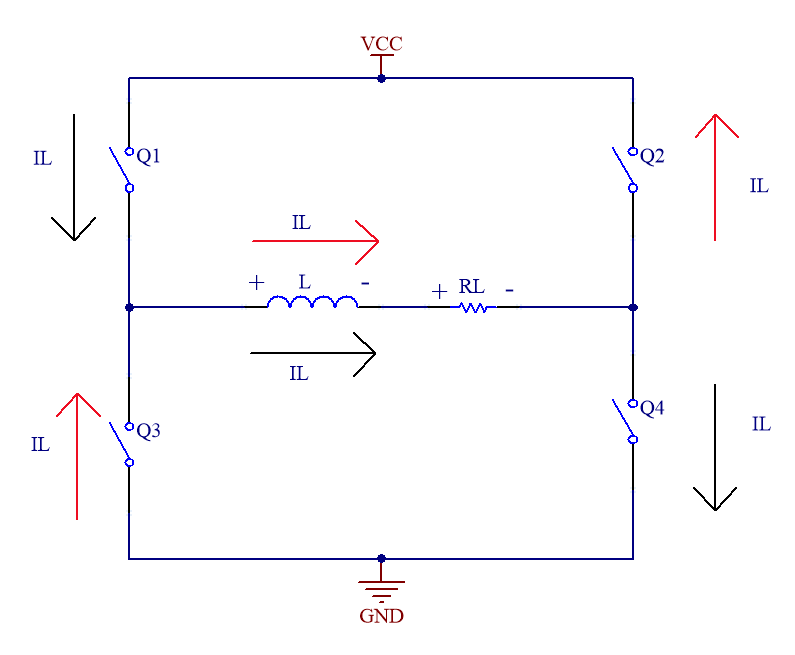
\includegraphics[width=\textwidth]{puente_con_llaves.png}
	\caption{Topología de puente H.}
	\label{fig:img_topologia_simplificada}
\end{figure}

Esta topología permite el control individual del estado de cada llave por medio de las señales de control ($S_x$). Cada una tiene dos estados posibles: abierto ($S_x=0$), no conduce corriente; y cerrado ($S_x=1$), conduce corriente sin caida de tensión en la llave. Las llaves se activan de a pares y, al combinar los valores de las señales de control de cada llave, se pueden generar distintas diferencias de potencial sobre el electroimán. A continuación se muestra una tabla con las posibles combinaciones de pares de llaves, y diferencia de potencial resultante en el electroimán ($V_L$):

\begin{table}[H]
	\begin{center}
		\begin{tabular}{| c | c | c | c | c |}
			\hline
			$S_1$ & $S_2$ & $S_3$ & $S_4$ & $V_L$ \\ \hline
			1 & 1 & 0 & 0 & 0 \\ \hline 
			1 & 0 & 1 & 0 & x \\ \hline 
			1 & 0 & 0 & 1 & $+V_{cc}$ \\ \hline 
			0 & 1 & 1 & 0 & $-V_{cc}$ \\ \hline 
			0 & 1 & 0 & 1 & x \\ \hline 
			0 & 0 & 1 & 1 & 0 \\ \hline 
		\end{tabular}
		\caption{Combinaciones de llaves}
		\label{tab_llaves}
	\end{center}
\end{table}

En la tabla \ref{tab_llaves} se observa que de todas las combinaciones posibles, solo dos generan una diferencia de potencial $\pm V_{cc}$ sobre el electroimán. Estas son  $S_1$ y $S_4$ cerrados y $S_2$ y $S_3$ abiertos para $V_L=+V_{cc}$, o con $S_2$ y $S_3$ cerrados y $S_1$ y $S_4$ abiertos para $V_L=-V_{cc}$. Al controlar el estado de las llaves alternando entre estas dos combinaciones, se logra una alimentación simétrica de la carga.

Debido a que solo se utilizan estas dos combinaciones, se puede reducir la cantidad de señales que controlan el sistema: $S_1=S_4$, $S_2=S_3$ y $S_1=\overline{S_2}$. Por lo tanto se define una nueva señal de control $S_T$ tal que $S_T=S_1=\overline{S_2}=\overline{S_3}=S_4$. El puente completo puede ser controlado por una sola señal, lo que simplifica el diseño de la etapa de lógica de control. Esta señal coincide con la entrada $V_h$ del bloque amplificador en la figura \ref{fig:img_diag-en-bloques-conH-y-Kin}.

Para esta aplicación en particular, la fuerza magnética es siempre en el mismo sentido, independientemente del sentido en que circule la corriente. Por lo tanto, se adopta como sentido de circulación positivo de izquierda a derecha como lo indican las flechas en la figura \ref{fig:img_topologia_simplificada}. 


% Esta topología permite la excursión negativa de la corriente mientras que mantiene en funcionamiento al estimador de posición.

\subsubsection{Funcionamiento del puente H}

Para poder obtener una forma de onda de corriente como la que se muestra en la figura \ref{fig:img_corriente_exponencial}, comenzando desde corriente nula, se debe controlar el estado de las llaves de la siguiente manera:


\begin{itemize}
	\item En principio se cierran las llaves $Q_1$ y $Q_4$ a la vez con $S_T=1$, generando un circuito entre $V_{CC}$, el electroimán y GND como indican las flechas negras en la figura \ref{fig:img_topologia_simplificada}. De esta forma, la corriente comienza a crecer con forma de exponencial negativa.
	\item Al llegar al límite superior de corriente ($I_{L_{MAX}}$), se debe conmutar el estado de la señal de control ($S_T=0$), de manera que $Q_1$ y $Q_4$ dejen de conducir, y comiencen a hacerlo $Q_2$ y $Q_3$. De esta manera, la corriente seguirá circulando en el mismo sentido como indican las flechas rojas, pero ahora la diferencia de potencial en los bornes del electroimán se opone al paso de la corriente, por lo que su magnitud comienza a decrecer.
	\item Una vez alcanzado el límite inferior de corriente ($I_{L_{MIN}}$), se vuelve a conmutar el estado de la señal de control ($S_T=1$) para que la corriente vuelva a crecer.
	\item Este ciclo se repite en régimen permanente para que el valor medio de la corriente generada coincida con la deseada. 
\end{itemize}

Es importante tener en cuenta que sólo dos llaves pueden encenderse a la vez, y esto debe realizarse de manera diagonal. Es decir, en la figura \ref{fig:img_topologia_simplificada}, $Q_1$ y $Q_4$ pueden estar encendidos, mientras que $Q_3$ y $Q_2$ están apagados, y viceversa. Esto es debido a que si se encendieran a la vez  $Q_1$ y $Q_3$ o  $Q_2$ y $Q_4$ se generaría un cortocircuito entre la fuente de alimentación y GND, produciendo una circulación de corriente elevada que podría dañar el sistema y la fuente de alimentación. Esta restricción será tenida en cuenta en el momento de diseñar el circuito encargado de controlar estas llaves.

El valor de tensión de la fuente de alimentación utilizada para el puente H está basado en la versión anterior del dispositivo, por lo que se utiliza $V_{CC} = 24\:V$.

\section{Elección y cálculo de parámetros del controlador}

En esta sección se determinarán los parámetros críticos para el correcto funcionamiento del controlador de corriente.

%\subsection{Cálculo de tensión de alimentación}

%Como se esta excitando a un sistema RL que posee una constante de tiempo ($\tau$) definida con una conmutación de tensión $\pm Vcc$, la elección de este ultimo valor determina la velocidad de respuesta que el sistema tendrá ante perturbaciones o cambios en el punto  de operación.

%La determinación del valor de la tensión de alimentación $V_{CC}$ a utilizar es importante ya que determina la velocidad con la que responde el sistema ante perturbaciones o a cambios en el punto de operación. Por lo tanto, se analiza qué valor de tensión de alimentación es requerida para lograr aumentar la corriente que circula por el electroimán lo suficientemente rápido para que pueda responder ante esas situaciones.
%
%Para ello, se plantea el caso en que el sistema se encuentra con un objeto de 1Kg suspendido a una distancia de 5mm y este cambia abruptamente a 30Kg. 
% 
%Las condicion inicial del problema es un objeto de 1Kg suspendido a una distancia de 5mm, por lo que por el electroimán estarán circulando 3.72A. La condición final es una masa 30Kg a 6mm, lo que resulta en una corriente de 24.48A. Por lo tanto, el sistema debe ser lo suficientemente rapido para aumentar la corriente 20.75A antes de que el objeto llegue a 5mm. 
%
%Nos dio un Vcc de 26.79 (con una inductancia para 4mm)
%Nos dio un Vcc de 24.4 (con una inductancia para 5mm)
%Nos dio un Vcc de 23.7 (con una inductancia para 6mm)
%\colorbox{red}{repetir cálculo con y=4}
%\begin{equation}
%	I_L(Y=4\:mm)[m=1\:kg]=3.72\:A  
%\end{equation}
%
%\begin{equation}
%	I_L(Y=5\:mm)[m=30\:Kg]=20.4\:A 
%\end{equation}
%
%Antes de llegar a un tiempo....T1
%%Es importante determinar cómo será la alimentación del controlador de corriente. Para hacerlo se debe tener en cuenta la velocidad de respuesta de la planta que está determinada por su constante de tiempo ($\tau$). Es decir, el sistema debe ser lo suficientemente rápido para modificar el valor medio de la corriente ante perturbaciones o cambios en el punto de operación. 
%
%
%
%Un caso a analizar es cuando, en régimen permanente, se modifica bruscamente la carga que esta levitando. En esta situación el sistema debe aumentar o disminuir la corriente de forma abrupta para evitar que el objeto se caiga. El caso de mayor exigencia se da cuando a una distancia máxima de referencia $Y_g=5\:mm$ se modifica de carga mínima ($1\:Kg$) a máxima ($30\:Kg$). Utilizando la ecuación \label{eq_corriente_peso} se obtiene que la corriente para ambos casos es de:
%
%Es importante tener en cuenta que la inductancia se consideró constante.
%
%
%
%
%Dado que el polo dominante ya está definido por el circuito RL del electroimán, la velocidad con que el sistema pueda alcanzar un valor de corriente elevado está determinado por el valor de la fuente de alimentación. La expresión teórica de la corriente es: 
%
%\begin{equation}
%	I_L(t)=\frac{V}{R_L} + (I_o-\frac{V}{R_L})*e^{-\frac{t}{\tau}}
%\end{equation}
%
%Donde:
%\begin{itemize}
%	\item V es la tensión de alimentación, que puede tomar valores $+V_{cc}$ y $-V_{cc}$.
%	\item $I_o$ es la corriente en el instante inicial.
%	\item $\tau$ es la constante de tiempo del electroimán.
%\end{itemize}
%
%Para encontrar la expresión del tiempo que tarda la corriente en alcanzar el valor máximo de corriente $i_{max}$ se reemplaza $I_{0}=2.9$ y se obtiene $T_{1}$. Esto da:
%
%\begin{equation}\label{eq_tiempo_de_subida}
%	T_1=-\tau*ln(\frac{V_{cc}-R*I_{max}}{V_{cc}-R*I_{0}})
%\end{equation}
%
%Cuando se modifique la carga del objeto ,es necesario que el tiempo de subida de corriente $T_1$ sea mucho menor al tiempo en que la carga llegue a la distancia máxima que el sistema soporta $Y=5mm$ aprox (que corresponde a $I_{max}$). Es decir que el objeto cae libremente un delta $\Delta Y= 1mm $. Utilizando la ecuación \ref{eq_caida_libre} se obtiene el tiempo (T) que tarda en desplazarse un objeto en caída libre una altura $\Delta Y$:
%
%\begin{equation}\label{eq_caida_libre}
%	T=\sqrt{\frac{2*\Delta Y}{g}}=\sqrt{\frac{2*1mm}{9.81}}=14,27\:ms
%\end{equation}
%
%Reemplazando este valor en la ecuación \ref{eq_tiempo_de_subida} se puede obtener el valor de tensión mínimo de $V_{CC}$ para que se alcance una velocidad de respuesta aceptable para que circule la corriente necesaria para que el objeto mantenga la posición deseada.
%
%El valor obtenido es $Vcc\geq21.6\:V$ por lo que se escoge un valor comúnmente utilizado de $24 V$.
%
%
%colorbox{Se puede decir cuanto da $T_1$ si tomamos 24V.}

\subsection{Cálculo de ancho de histéresis}

%Como se mencionó, se desea controlar la fuerza ejercida a partir del valor medio de la corriente. Por lo tanto, las variaciones en torno a dicho valor medio no deben generar variaciones significativas en la fuerza magnética. Por ello, se debe elegir un ancho de histéresis tal que la frecuencia de conmutación resultante sea filtrada por la dinámica de la planta. Un valor de al menos 100 veces mayor que la frecuencia del polo de la planta obtenida en \ref{eq_transferencia_planta_m} serìa suficiente. Este se ubica en $70\:r/s$, lo que resulta en que se debe conmutar a una frecuencia de $\omega_{sw}>=7000\:r/s$, y expresada en Hz resulta $F_{sw}>=1\:kHz$.

Al trabajar en conmutación se está excitando al sistema, en estado estacionario, con una onda cuadrada en tensión. Como se mencionó previamente, la forma de onda de la corriente debe ser triangular de forma que esta oscile sobre un valor medio generando una fuerza constante con pequeñas variaciones que no afectan la dinámica de la planta.

Para lograr esto, la frecuencia de conmutación debe ser al menos 100 veces mayor que la frecuencia del polo de la planta obtenida en \ref{eq_transferencia_planta_m}.
De esta forma la dinámica de la planta y la respuesta a los transitorios no se ven afectadas.  Por lo tanto, dado que el polo se ubica en $70\:r/s$  se debe conmutar a una frecuencia de $\omega_{sw}\geq7000\:r/s$ (expresada en Hz resulta $F_{sw}\geq1\:kHz$).

Por lo tanto, como la frecuencia mínima es $F_{sw}$, y considerando que el tiempo en que crece la corriente es igual al que decrece, se obtiene que el tiempo máximo que puede tener la sección creciente de la corriente es igual a $t_{max}=500\:us$. 

A partir de la expresión \ref{eq_corriente_temporal_cond_iniciales} se puede obtener el valor máximo de \textsl{ripple} cuando $t=t_{max}$, considerando que la corriente inicial es $I_{min}$ y que la corriente final es $I_{min}+\Delta I_L$

\begin{equation} \label{eq_delta_i}
	I_{min}+\Delta I_{L_{max}}=\frac{V_{CC}}{R_L}+(I_{min}-\frac{V_{CC}}{R_L})*e^{-\frac{t_{max}}{\tau}}
\end{equation}

De la ecuación \ref{eq_delta_i} se obtiene el valor máximo que se le puede asignar a $\Delta I_L$. 

\begin{equation} \label{eq_delta_i_2}
	\Delta I_{L_{max}}=6.06*10^{-3}*(\frac{V_{CC}}{R_L}-I_{min})
\end{equation}

El controlador de corriente tendrá una corriente media variable entre $0\:A$ y $30\:A$, por lo que se debe satisfacer la expresión \ref{eq_delta_i_2} para cualquier valor de corriente dentro de ese rango. De esta forma, se plantean dos casos: $I_{min}=0\:A$ e $I_{min}=30\:A$. Para el primero se obtiene que $\Delta I_{L_{max}}=727\:mA$ y en el segundo $\Delta I_{L_{max}}=541.6\:mA$. Por lo tanto, se elige un ancho de histéresis de $500\:mA$ ya que cumple las dos condiciones.

\subsection{Cálculo de ganancia de entrada}

Como se observa en el diagrama en bloques de la figura \ref{fig:img_diag-en-bloques-conH-y-Kin}, la etapa de entrada consiste en la ganancia $K_{in}$ y el restador con la señal realimentada. El objetivo es que una tensión de referencia en la entrada entre $0\:V$ y $5\:V$ se corresponda de manera lineal con una corriente de salida entre $0\:A$ y $30\:A$ (en valor medio). Por lo tanto, se obtiene una ganancia del controlador de corriente de $6\:A/V$. Si bien aún no se eligió el sensor de corriente que será utilizado, puede considerarse su ganancia de contínua $H(s=0)$, denominada $H_0$. En la expresión \ref{eq_kin} se muestra la ganancia de entrada en función de $H_0$ para poder calcularla una vez elegido el sensor.

\begin{equation} \label{eq_kin}
	K_{in}=\frac{30\:A*H_0}{5\:V}=6*H_0 
\end{equation}

%Como se ve en el diagrama en bloques de la figura \ref{fig:img_diag-en-bloques-conH-y-Kin} la etapa de entrada que consiste en la ganancia $K_{in}$ y el restador con la señal realimentada. El objetivo es que una tensión de referencia en la entrada entre $0\:V$ y $5\:V$ se corresponda de manera lineal con una corriente de salida entre $0\:A$ y $30\:A$ (en valor medio). Por lo tanto, se obtiene una ganancia del controlador de corriente de $6\:A/V$. Dado que la ganancia del sensor HO15-NP \cite{HO15-NP} es de $H(s) = 53.3\:mV/A$ se puede calcular la ganancia de entrada como:
%
%\begin{equation}
%	K_{in}=\frac{30\:A*53.3\:mV/A}{5\:V}=0.32 
%\end{equation}
%
%La salida de esta etapa, al igual que la tensión de salida del sensor de efecto Hall, se polarizan en un punto de operación de $2.6\:V$.
\section{Diseño circuital del controlador de corriente}

En esta sección se realiza la implementación circuital de cada bloque planteado en la sección anterior, teniendo en cuenta consideraciones prácticas para cada uno.


\subsection{Elección del sensor de corriente}

Como se mencionó previamente es necesario realizar una medición sobre la corriente que circula por el bobinado del electroimán para que luego el controlador pueda actuar en consecuencia. Es importante conocer tanto su valor medio como su \textsl{ripple}. Es por ello que se debe idear una estrategia de medición que represente correctamente esta forma de onda cuyo valor medio puede alcanzar valores desde $0\:A$ hasta $30\:A$ con un \textsl{ripple} de $500\:mA$.

En esta sección se analizan dos alternativas para lograr este objetivo. La primera mediante una resistencia en serie al electroimán y la segunda utilizando un sensor de efecto Hall.


\subsubsection{Análisis de medición de corriente mediante resistencia shunt}

Una forma de medir la corriente es utilizar una resistencia de valor $R_s$ en serie con el electroimán como se muestra en la figura \ref{fig:img_puente_con_rshunt}, y medir en sus terminales la diferencia de tensión generada por la corriente. A partir de esta tensión ($V_s-V_a$) se puede utilizar la ley de Ohm para conocer el valor de corriente:

\begin{equation}
	I_L=\frac{V_s-V_a}{R_s}
\end{equation}

\begin{figure}[H]
	\centering
	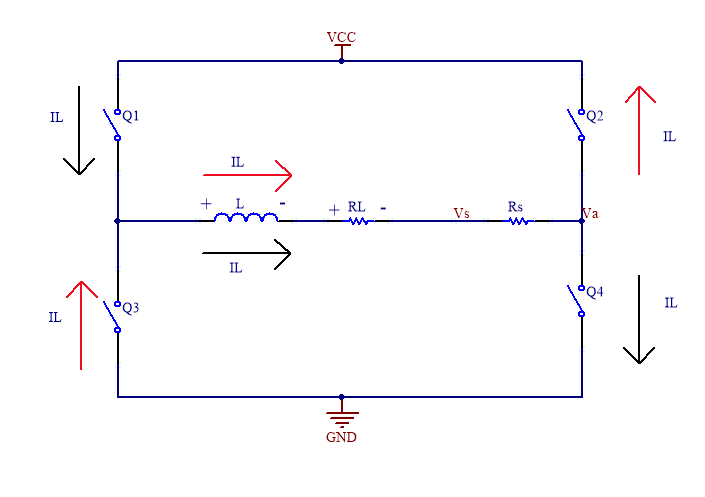
\includegraphics[scale=0.6]{puente_con_rshunt.png}
	\caption{Puente H con resistencia de sensado de corriente (Rs).}
	\label{fig:img_puente_con_rshunt}
\end{figure}

Como se observa en el diagrama en bloques \ref{fig:img_diag-en-bloques-conH-y-Kin}, la ganancia de realimentación $H(s)$ corresponde al valor de la resistencia $R_s$.

Si bien es posible utilizar este método para medir la corriente, se presentan algunos inconvenientes en su implementación circuital que se mencionan a continuación.

El primero es que al agregar una resistencia en serie al electroimán se introduce una mayor disipación de potencia en el sistema. Para intentar reducir los efectos de este problema se podría elegir un valor de resistencia lo suficientemente bajo para que su consumo de potencia sea despreciable. Por ejemplo, si se adopta una resistencia de $10\:m\Omega$ el valor de pérdidas de potencia es de $4\:W$, que es un valor aceptable frente a al consumo del electroimán que es de $80\:W$ (considerando una corriente de $20\:A$).

El segundo inconveniente es que se altera la dinámica de la planta, ya que la constante de tiempo cambia a $\tau=\frac{L}{R_L+R_s}$. Sin embargo, el electroimán presenta una resistencia interna de $0.2\:Ohm$, por lo que una resistencia de sensado con valor $10\:mOhm$ no afectaría en gran medida su comportamiento.

El tercero es que se debe realizar una medición de tensión flotante. Esto se debe a que la resistencia, al estar en serie con el electroimán, no tiene ningún punto de medición referido a masa. Por lo tanto, se debe utilizar un amplificador que mida tensión en modo diferencial para luego obtener una señal en modo común. El inconveniente que se presenta es que cada uno de los puntos de medición se encuentra a un alto potencial respecto de masa y, además, este cambia en cada conmutación. Esto genera que durante los transitorios de conmutación haya ruido en la medición diferencial.

Debido a que se requiere medir el valor de corriente sin que el ruido de modo común altere la medición, se propone analizar otra alternativa que sea inmune a dicho efecto.


\subsubsection{Análisis de medición de corriente mediante sensor de efecto Hall}

Dado que la medición con una resistencia de shunt introduce ruido ocasionado por la conmutación de las llaves, se plantea como alternativa utilizar un sensor de efecto Hall. Estos dispositivos miden el campo magnético generado por la corriente, entregando a su salida una tensión proporcional a ésta. La principal ventaja que presentan es que el campo magnético medido sólo es sensible a las variaciones de corriente y no a las conmutaciones de tensión.

Existen una gran variedad de estos sensores en el mercado, cada uno con diferentes características. A continuación se mencionan los criterios que se tendrán en cuenta para la elección del sensor:

\begin{itemize}
	\item Debe ser capaz de medir y presentar una transresistencia lineal entre $0\:A$ y $30\:A$.
	\item El ancho de banda debe ser mucho mayor al polo de la frecuencia de conmutación del controlador de corriente ($1\:kHz$) para poder conservar la forma de onda de la corriente triangular a medir. Por lo tanto, debe ser al menos de $100\:kHz$.	
\end{itemize}

A partir de estas características se decidió utilizar el sensor HO 15-NP-0000 \cite{HO15-NP}. Este permite medir una corriente de $\pm 37.5\:A$ con un ancho de banda de $250\:kHz$ y una transresistencia de $H(s)=H_0=53.33\:mV/A$ en todo  el rango de corriente. Además, presenta alta inmunidad a interferencias externas. Por otro lado, requiere una fuente de alimentación simple de $5\:V$.

Este sensor tiene la capacidad de medir tanto corrientes en sentido positivo, como negativo. Para ello admite una tensión de operación ($V_{op}$) de $2.5\:V$, la cual se corresponde a la salida cuando la corriente es nula. Cuando la circulación de corriente es positiva, la salida del sensor resulta en una tensión mayor a $2.5\:V$ y, para negativas, menor.

De esta forma, el bloque $H_0$ de realimentación queda definido como:

\begin{equation}
	H_0=\frac{V_{IL_{feed}}}{I_L}=53.33 \:\frac{mV}{A}
\end{equation}

\subsubsection{Conexión de sensor en el puente}
\colorbox{red}{esto se puede modificar o sacar si quieren, pero me parece que es importante marcar la señal Vsns que después la usamos en los operacionales}

El sensor se conecta dentro de la fuente de alimentación de la manera que se muestra en la figura \ref{fig:img_conexion_sensor}. Entre sus conexiones mas relevantes se encuentran la entrada de alimentación (pin 1), la entrada de corriente del electroimán (pines 8, 9, 10), la salida de corriente (pines 11, 12, 13), la entrada de tensión de referencia (pin 4) y la señal de salida $V_{sns}$ (pin 3).

\begin{figure}[H]
	\centering
	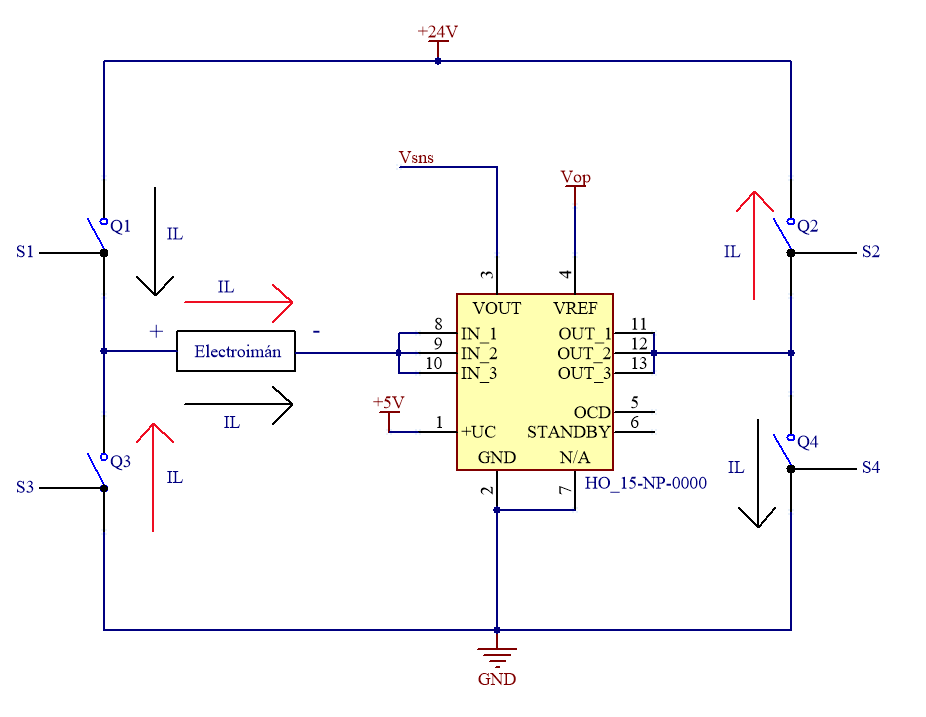
\includegraphics[scale=1]{conexion_sensor_hall.png}
	\caption{Sensor de corriente dentro del puente H.}
	\label{fig:img_conexion_sensor}
\end{figure}

La señal $V_{sns}$ está dada por la ecuación siguiente:

\begin{equation}
	V_{sns}=I_L*H_0+V_{op}
\end{equation}

\colorbox{red}{sacar capacitores de desacople}

\subsection{Elección de llaves de conmutación} \label{sec_eleccion_llaves}

Las llaves de conmutación ($Q_1$, $Q_2$, $Q_3$ y $Q_4$) que se muestran en la figura \ref{fig:img_topologia_simplificada} son llaves ideales que, en la práctica, se implementan por medio de dispositivos semiconductores cuyas características no son ideales. Sin embargo se pueden elegir componentes que se aproximen al comportamiento ideal: resistencia nula al estar en conducción e infinita al estar en estado abierto. De esta forma no se modifica la dinámica de la planta y se reduce la disipación de potencia.

Para la implementación de las llaves se analiza la utilización de dispositivos semiconductores pertenecientes a la clase transistores. En el mercado existe una amplia variedad de ellos, entre los que se encuentran los transistores bipolares de juntura (TBJ), los transistores de efecto de campo metal-oxido-semiconductor (MOSFET), entre otros. Cada uno de ellos posee características distintivas que lo hacen más o menos apropiado para cada aplicación en particular. 

Estos dispositivos presentan diferencias en cuanto a su mecanismo interno de funcionamiento y forma de utilización. En la tabla \ref{tab_MOSFETvsBJT} se resumen las características principales de cada tipo:

\begin{table}[H]
	\begin{center}
		\begin{tabular}{| c | c | c |}
			\hline
			Tipo & $BJT$ & $MOSFET$\\ \hline
			Manejo del \textsl{gate} & Por corriente & Por voltage \\ \hline 
			%Características de Voltaje (Encendido) & $V_{ce}$ bajo & presenta $R_{ds}$ \\ \hline 
			Velocidad de conmutación & Lento & Rápido \\ \hline 
			Diodo antiparalelo & No presente & Presente \\ \hline 
			Caída de tensión en conducción & Depende de tensión  $V_{CE}$ & Depende de resistencia $R_{ds}$ \\ \hline 
			Dirección de corriente & En un solo sentido & En ambos sentidos \\ \hline 
		\end{tabular}
		\caption{BJT vs MOSFET}
		\label{tab_MOSFETvsBJT}
	\end{center}
\end{table}

Dadas las características de cada uno mostradas en la tabla \ref{tab_MOSFETvsBJT}, resulta conveniente que el dispositivo elegido permita la circulación de corriente en ambos sentidos (o que no requiera del agregado de componentes externos para lograrlo), permita rápidas conmutaciones y dispongan de diodos antiparalelo que permitan la circulación de corriente para cargas inductivas al momento de conmutación de las llaves. Por lo tanto, se decide utilizar la tecnología MOSFET.

Para la elección del modelo que se utilizará se tienen en cuenta los siguientes requerimientos: debe soportar una corriente ($I_{D}$) mayor a $30\:A$, una tensión entre \textsl{drain} y \textsl{source} ($V_{DS}$) mayor a $24\:V$, y baja resistencia en estado de conducción ($R_{DS_{ON}}$).


\colorbox{red}{Agregar datasheet del MOSFET?}

Por lo tanto, se decide utilizar los MOSFET IPB160N04 ya que, ademas de haber sido probados en el prototipo anterior, cumplen con los requerimientos de corriente: soportan una $I_{D_{MAX}}=160\:A$, una tensión $V_{DS_{MAX}} = 40\:V$ y una $R_{ds} = 1.6 \:m \Omega$. Estos transistores son de tipo N y, para que estén en estado de conducción con la $R_{ds}$ especificada anteriormente, debe aplicarse una tensión entre \textsl{gate} y \textsl{source} mínima de $V_{gs}= 7\:V$.

Para lograr una conmutación sincronizada de los MOSFET se necesita un dispositivo que permita activar los pares de transistores de forma sincronizada con una tensión adecuada en sus \textsl{gates}. Este dispositivo tiene el nombre de MOSFET \textsl{driver} e integran varias funcionalidades útiles para el control de los mismos. 

\subsubsection{Componentes auxiliares para los MOSFET} \label{sec_auxiliares_mosfet}


Para el correcto funcionamiento de los MOSFET es necesario agregar circuitería de protección y acondicionamiento como se muestra en la figura \ref{fig:img_capacitores-puenteH}.


\begin{figure}[H]
	\centering
	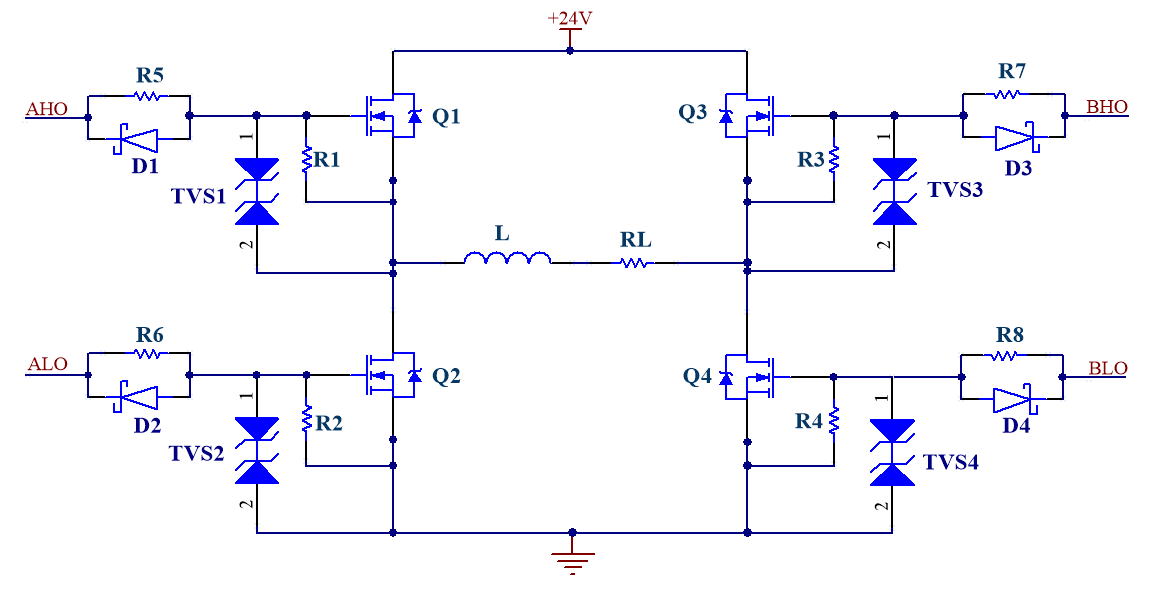
\includegraphics[scale=0.4]{Capacitores-puenteH.png}
	\caption{Puente H.}
	\label{fig:img_capacitores-puenteH}
\end{figure}

\colorbox{red}{Dejar S1, S2, ...}

\subsubsubsection{Resistencias de descarga de \textsl{gate}}\label{sec_res-gate}

\noindent Se colocan resistencias que conectan el \textsl{gate} y el \textsl{source} de cada MOS en el puente H. Estas se observan en la figura como $R_1$, $R_2$, $R_3$ y $R_4$ y tienen el objetivo de evitar que el \textsl{gate} del MOSFET se encuentre cargado cuando el circuito se enciende y el \textsl{driver} de corriente aún no puede descargarlo. Además, ayuda a evitar que se encienda el MOSFET por ruido acoplado capacitivamente. 

\noindent Se elige un valor de $4.7 \:k\Omega$  para las resistencias debido a que permite que el \textsl{gate} se descargue en un tiempo rápido, sin generar un consumo de corriente elevado de la señal de control del \textsl{gate}.

\subsubsubsection{Protección de sobretensión del \textsl{gate}}

\noindent El \textsl{gate} de los MOS es sensible a las sobretensiones: soporta como máximo $\pm 20\:V$. Una descarga electrostática (ESD) puede sobrepasar ampliamente este valor de tensión y dañar el MOS al acercar la mano o la sonda del osciloscopio. Para protegerlo se coloca un diodo TVS entre el \textsl{gate} y \textsl{source} de cada transistor, de manera de limitar la tensión que se desarrolla en el \textsl{gate} a un valor seguro. Estos se observan como $TVS_1$, $TVS_2$, $TVS_3$ y $TVS_4$ en la figura \ref{fig:img_capacitores-puenteH}. Se eligen los TVS SMAJ15 con una tensión bidireccional de $\pm 15\:V$.
\colorbox{red}{hacer referencia a hoja de datos}

\subsubsubsection{Resistencia y diodo en serie al \textsl{gate}}

Debido a que existen inductancias parásitas en el \textsl{gate}, y que este tiene una impedancia de entrada capacitiva, se forma un circuito resonante LC. Al hacer una conmutación de tensión se pueden generar oscilaciones en la señal de control, lo que puede provocar una incorrecta activación del MOSFET. Para reducir este inconveniente se agrega resistencia en serie al \textsl{gate} en el circuito ($R_5$, $R_6$, $R_7$ y $R_8$), con el objetivo de amortiguar las oscilaciones. Esto trae la desventaja de que hace mas lenta la velocidad de encendido y apagado. Por otro lado, como se desea apagar el MOSFET en el menor tiempo posible, se genera un camino de descarga del \textsl{gate} a través de un diodo en paralelo a la resistencia ($D_1$, $D_2$, $D_3$ y $D_4$).

Para el diseño del circuito impreso de esta etapa se propone en principio utilizar resistencias de 0Ohm y que, en caso de resultar necesario, puedan ser reemplazadas por un valor de resistencia adecuado. 

\subsection{Elección y análisis del \textsl{driver} de corriente}

Como se mencionó en la sección \ref{sec_eleccion_llaves}, se necesita agregar al circuito un \textsl{driver} de MOSFETs. Para ello se elige el \textsl{driver} HIP4081A \cite{HIP4081A_FN3659}. Este dispositivo requiere una fuente de alimentación simple de $12\:V$ y permite el control de un puente completo a partir de señales de control con niveles lógicos entre $0\:V$ y $5\:V$. 

La topologia del puente H con el \textsl{driver} puede verse en la figura \ref{fig:img_topologia-puenteH} donde las salidas de control del HIP4081A se conectan a los \textsl{gates} de los MOSFET.

\begin{figure}[H]
	\centering
	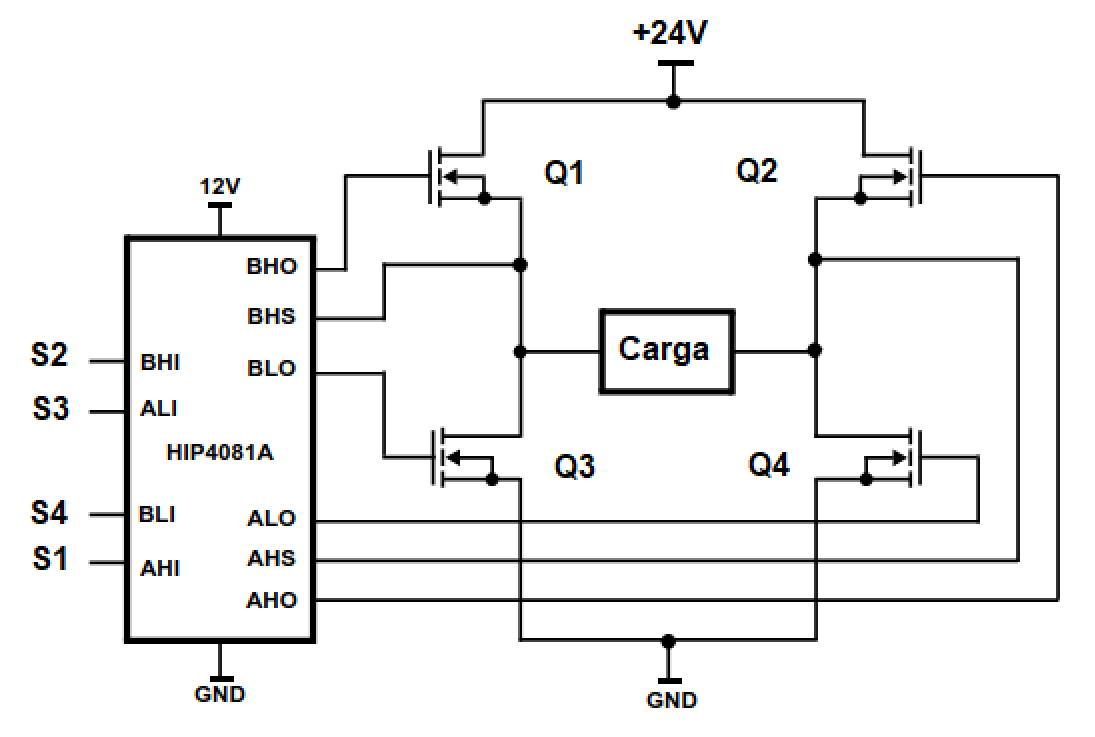
\includegraphics[scale=0.7]{Topologia-puenteH.png}
	\caption{Topología elemental del puente H.}
	\label{fig:img_topologia-puenteH}
\end{figure}

\colorbox{red}{modificar cosas de la imagen como Vcc, load, etc..., agregar señales s1,s2,s3,s4}

Dado que los cuatro MOSFET utilizados para el puente H son de tipo N. Para que estos puedan funcionar correctamente en conmutación es necesario que en el estado ON, la diferencia de tensión entre \textsl{gate} y \textsl{source} sea mayor o igual a $V_{gs min}(ON) = 7\:V$. Esto no es un problema para los dos MOS inferiores del puente H ($Q_2$ y $Q_4$), ya que la tensión en \textsl{source} está fijada en GND y el \textsl{driver} puede aplicar $12\:V$ al \textsl{gate} (superando los $7\:V$ entre \textsl{gate} y \textsl{source}). El problema radica en los transistores superiores del puente H, ya que la tensión en \textsl{source} varía entre $0\:V$ y $24\:V$, por lo que en el \textsl{gate} debería haber, por lo menos, $31\:V$ con respecto a GND. Sin embargo, la tensión máxima disponible entregada por la fuente es de $24\:V$. Para resolver este problema se hace uso de una funcionalidad que presenta el \textsl{driver} HIP4081A: entregar una diferencia de tensión mayor a $+24\:V$ a partir de una tensión flotante con una configuración de \textsl{bootstrap}.

En la figura \ref{fig:img_bootstrap} se observa solo una de las mitades del puente H (lado A) junto con las señales de control provistas por el \textsl{driver} HIP4081A.  El análisis para la otra mitad es análogo, por lo que se evita por simplicidad. La implementación del \textsl{bootstrap driver} permite obtener en el \textsl{gate} del MOS superior, una tensión de $36\:V$ respecto a GND, de manera que se logra una diferencia de tensión mayor a $7\:V$ entre \textsl{gate} y \textsl{source}. 
\colorbox{red}{Ver si podemos aclarar que S1 es AHO, etc}
\begin{figure}[H]
	\centering
	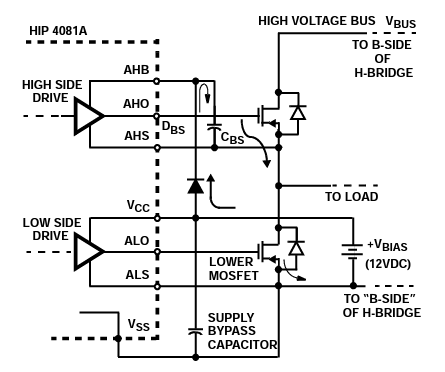
\includegraphics[scale=0.7]{Bootstrap.png}
	\caption{Configuración \textsl{bootstrap} simplificada.}
	\label{fig:img_bootstrap}
\end{figure}

El \textsl{bootstrap driver} consiste en un capacitor ($C_{BS}$), un diodo, y la circuitería interna del HIP4081A. Para garantizar el correcto funcionamiento del \textsl{bootstrap}, al encender el sistema, la secuencia de inicio del HIP4081A enciende las dos salidas de la parte inferior del puente H: ALO y BLO con el fin de encender $Q_2$ y $Q_4$ durante un tiempo que se conoce como periodo de refresco de \textsl{bootstrap}. De esta forma, los capacitores de \textsl{bootstrap} de ambos lados quedan conectados entre $12\:V$ y GND y se pueden cargar completamente. Durante este tiempo, las salidas a los \textsl{gates} AHO y BHO se mantienen en bajo continuamente lo que asegura que no se produzca corriente de cortocircuito durante el período nominal de refresco del \textsl{bootstrap}. Una vez finalizado, las salidas responden normalmente al estado de las señales de entrada de control.

Para comprender su funcionamiento se hará un breve análisis del sistema. Para ello, se parte de la suposición de que el sistema se encuentra en funcionamiento: con el transistor $Q_2$ encendido (ALO = $V_{CC}$), $Q_1$ apagado (AHO = AHS = $0\:V$) y la corriente circulando de izquierda a derecha como lo indica la figura \ref{fig:img_bootstrap}. En ese caso, el capacitor $C_{BS}$ se carga a $12\:V$, ya que en un terminal tiene la fuente de $12\:V$ (a través del diodo $D_{BS}$) y el otro está conectado a GND por medio de $Q_2$.

Una vez que se apaga el transistor inferior, empieza a transcurrir el tiempo muerto. Debido a que la carga es inductiva, el valor medio de la corriente mantiene su sentido y circula por los diodos antiparalelos del MOS inferior del lado A y el superior del lado B. Esto provoca que el \textsl{source} del MOS superior del lado A tenga una tensión negativa igual a la caída de tensión en directa del diodo antiparalelo de $Q_2$. 

Una vez finalizado el tiempo muerto, se enciende $Q_1$. Para ello, la señal AHO se pone en nivel alto. Durante el tiempo que $Q_1$ pasa de estar apagado a encendido, la tensión en el \textsl{source} cambia de $-V_d$ a $V_{bus}$ de manera gradual mientras se carga el \textsl{gate}, y AHO pasa a ser igual a AHB, que es igual a la tensión entregada por el capacitor de \textsl{bootstrap} sumada a la tensión en el \textsl{source} de $Q_1$. De esta manera se logra una tensión de $36\:V$ con respecto a GND en el \textsl{gate} y genera una diferencia entre \textsl{gate} y \textsl{source} de $12\:V$.

Para lograr un funcionamiento adecuado del \textsl{bootstrap} es necesario dimensionar correctamente al capacitor $C_{BS}$ con el fin de que pueda proveer la carga suficiente durante el tiempo en el que el MOS esté encendido.

\subsubsection{Tiempo muerto}

\noindent Para evitar generar un cortocircuito durante la conmutación de los transistores, el \textsl{driver} HIP4081A permite configurar un tiempo muerto que debe transcurrir desde que se apaga un transistor y se enciende el próximo. Esto se configura mediante dos resistencias conectadas a sus pines LDEL y HDEL.

\noindent Para saber el tiempo muerto necesario, debe conocerse el tiempo que tarda en apagarse un MOSFET IPB160N04. De \cite{IPB160N04} se obtiene que este tiempo es de $63\:ns$ (teniendo en cuenta el $T_{OFF}$ y el $T_{FALL}$). Por lo tanto, se elige que el tiempo muerto sea de $100\:ns$ para tomar un margen.

\noindent Según la hoja de datos del HIP4081A, para obtener ese tiempo muerto, las resistencias en HDEL y LDEL deben ser $200\:k\Omega$.

\subsection{Dimensionamiento de capacitor de \textsl{bootstrap}}\label{sec_cap_bootstrap}

\noindent Para el dimensionamiento de los capacitores de \textsl{bootstrap} se tuvieron en cuenta sugerencias y procedimientos descriptos en \cite{HIP4081A_AN9405} y \cite{HIP4081A_FN3659}.

Para encender un NMOS es necesario proveer corriente a su \textsl{gate} hasta cargar las capacidades parásitas entre \textsl{gate-source} y \textsl{gate-drain}. Una vez cargadas, el MOS queda en estado encendido y no consume más corriente en el \textsl{gate}. En el caso de los MOS del lado superior, esta corriente proviene del capacitor de \textsl{bootstrap}.

En la sección \ref{sec_res-gate} se agregaron resistencias de protección entre \textsl{gate-source}. Debido a la diferencia de tensión entre \textsl{gate-source}, se genera una corriente constante en estas resistencias durante el tiempo que el MOS esté encendido, que también debe ser provista por el capacitor de \textsl{bootstrap}.

\noindent Cuando el MOSFET \textsl{driver} recibe una entrada que activa un MOS del lado superior, este comienza a cargar el \textsl{gate} con ayuda de la tensión que brinda el capacitor de \textsl{bootstrap} asociado a ese MOS. El capacitor de \textsl{bootstrap} entrega energía durante la carga del \textsl{gate} y durante todo el tiempo que el MOS esté activo (debido a la resistencia $R_{GS}$). Para poder recargar el capacitor, debe esperarse a que el \textsl{driver} reciba la entrada necesaria para apagar el MOS. Debido a que la implementación del \textsl{driver} de corriente utiliza un controlador por histéresis, no es posible asegurar que haya una conmutación en un periodo regular.

\noindent Para poder asegurar un período de conmutación constante y conocido se agrega un bloque que superpone una conmutación de alta frecuencia a la señal de control que ingresa al MOSFET \textsl{driver}. De esta manera se producen conmutaciones en un intervalo regular que permiten la carga de los capacitores de \textsl{bootstrap}. El diagrama en bloques resultante se muestra en la figura \ref{fig:img_diag-en-bloques-con-oscilador}. 

\begin{figure}[H]
	\centering
	\scalebox{0.8}{%importo el bloque de histeresis que definí en otro archivo
%esto es para poder dibujar flechitas en la histeresis usando ->-
\tikzset{->-/.style={decoration={
			markings,
			mark=at position .5 with {\arrow{>}}},postaction={decorate}}}

%aca se define el dibujito de la histeresis uniendo lineas
\def\hist{
	\tikz[remember picture,overlay]{
		%dibujamos los ejes. stealth es para las flechas
		\draw [stealth-stealth] (-1,0) -- (1,0) node[pos=1, yshift=0.5em]{${\scriptstyle e}$};  %eje x
		\draw [stealth-stealth] (0,-0.8)--(0,0.8) node[pos=0.9, xshift=0.8em]{${\scriptstyle V_L}$}; %eje y
		
		%esto es para dibujar los tramos de la histeresis
		\draw [->-] (-0.7,-0.4)-- (0.3,-0.4);
		\draw  [->-] (0.3,-0.4) -- (0.3,0.4); 
		\draw [->-] (0.7,0.4) --(-0.3,0.4);
		\draw [->-] (-0.3,0.4) -- (-0.3, -0.4);
}}

\tikzset{%
	buffer/.style={
		draw,
		shape border rotate=270,
		regular polygon,
		regular polygon sides=3,
		fill=blue!20,
		node distance=2cm,
		minimum height=4em
	}
}

%Acá se define eñ diagrama en bloques completo
\begin{tikzpicture}[auto, node distance=2.5cm,>=latex']
% We start by placing the blocks
\node [input, name=input] {};
\node [block, right of=input] (Kin) {$K_{in}$};
\node [sum, right of=Kin, node distance=2cm] (sum) {};
\node [block, right of=sum] (controller) {\histvh};
\node [draw,circle, fill=blue!20, right of=controller](multiplier){X};
\node [coordinate, above of=multiplier, node distance=1cm](osc) {}; 
\node [buffer, right of=multiplier, node distance=2cm](buffer){};
\node [coordinate, above of=buffer, node distance=1cm](Vcc){};
\node [coordinate, below of=buffer, node distance=1cm](Vee){};
\node [block, right of=buffer, 
node distance=3.5cm] (system) {${\displaystyle\frac{1}{s*L(Y_g)+R_L}}$};
% We draw an edge between the controller and system block to 
% calculate the coordinate u. We need it to place the measurement block. 
\draw [->] (controller) -- node[name=u]{$V_h$} (multiplier);
\draw [->] (multiplier) -- node{$V_{sw}$}(buffer);
\draw [->] (osc) -| node{$F_{aux}$} (multiplier);
\draw (Vcc) -| node{$V_{cc}$} (buffer);
\draw (Vee) -| node[right]{$-V_{cc}$} (buffer);
\draw [->] (buffer) -- node {$V_L$} (system);
\node [output, right of=system] (output) {};
\node [block, below of=u, node distance=3cm] (measurements) {H(s)};

% Once the nodes are placed, connecting them is easy. 
\draw [draw,->] (input) -- node[pos=0.1]{$V_{IL_{ref}}$} (Kin);
\draw [draw,->] (Kin) -- node[pos=0.9]{$+$} (sum);
\draw [->] (sum) -- node {$e$} (controller);
\draw [->] (system) -- node [name=y] {$I_L$}(output);
\draw  (y) |- (measurements);
\draw [->] (measurements) -| node[pos=0.99] {$-$} node[above, pos=0.9, right] {$V_{IL_{feed}}$} (sum); %node [near end] {$I_{L_{feed}}$} 
\end{tikzpicture}





}
	\caption{Diagrama en bloques completo del controlador de corriente}	\label{fig:img_diag-en-bloques-con-oscilador}
\end{figure}

\noindent Se adopta una frecuencia de conmutación auxiliar de $F_{sw}=50\:kHz$ y se hace variar el ciclo de trabajo de la señal $V_{sw}$ entre dos valores. Para la carga del inductor se definió que el ciclo de trabajo sea del 90\% mientras que para la descarga sea del 10\%.

\colorbox{red}{ver de mejorar el parrafo de arriba, de última fue..}

%
%Como hay una corriente que circula constantemente desde el capacitor de bootstrap hacia las resistencias de Gate-source, es necesario limitar el tiempo màximo que puede quedar encendido un transistor. Debido al funcionamiento del controlador por histéresis, no se puede asegurar que haya una conmutación a intervalos regulares... Es por ello que se decide modificar levemente el diagrama en bloques \ref{fig:img_diag-en-bloques-conH-y-Kin} de manera de superponer una conmutación de alta frecuencia a la señal de control de las llaves. 



\noindent Por otro lado, el capacitor debe entregar corriente al diodo de \textsl{bootstrap} cuando este queda en inversa ($I_{DR}$). El componente elegido para este diodo es el RSX205LAM30TR \colorbox{red}{Agregamos la hoja de datos?}. También debe entregar una corriente de fuga al circuito integrado HIP ($I_{QBS}$). Esta última se desprecia ya que es compensada internamente por la bomba de carga del HIP.

\noindent Por lo tanto, para poder dimensionar correctamente el capacitor de \textsl{bootstrap} es necesario tener en cuenta todos los efectos mencionados anteriormente. Para ello se parte planteando la carga que almacena este capacitor:

\begin{equation} \label{eq_carga-cap-bootstrap}
	Q_{BS}=C_{BS}*\Delta V_{BS}
\end{equation}

\noindent En la ecuación \ref{eq_carga-cap-bootstrap}, $Q_{BS}$ es la carga total del capacitor de \textsl{bootstrap}, $C_{BS}$ su capacidad, y $\Delta V_{BS}$ es la diferencia de  tensión entre sus terminales. 

\noindent Para evitar sufrir una caída de tensión tal que afecte el encendido de los MOS, es necesario que $Q_{BS}$ pueda abastecer también al \textsl{gate}, al diodo en inversa y a la resistencia entre \textsl{gate-source}. Por lo tanto:

\begin{equation} \label{eq_carga-cap-bootstrap2}
	Q_{BS} > Q_G + Q_{RR} + \frac{I_{DR}+I_{GS}}{F_{sw}}
\end{equation}

\noindent Donde:
\begin{itemize}
	\item $Q_G$ = Carga total que se debe entregar al \textsl{gate} del MOS.
	\item $Q_{RR}$ = Carga entregada al diodo en inversa durante el tiempo de recuperación (cuando pasa de modo conducción a inversa).
	\item $I_{DR}$ = Corriente de fuga del diodo en inversa.
	\item $I_{GS}$ = Corriente que circula por la resistencia de \textsl{gate-source}.
	\item $F_{sw}$ = frecuencia de conmutación.
\end{itemize}


\noindent Por lo tanto, al reemplazar la ecuación \ref{eq_carga-cap-bootstrap} en la \ref{eq_carga-cap-bootstrap2} resulta:


\begin{equation} \label{eq_cap-bootstrap}
	C_{BS} > \frac{Q_G+Q_{RR} + \frac{I_{DR}+I_{GS}}{F_{sw}}}{\Delta V_{BS}}
\end{equation}

\noindent Según la hoja de datos \cite{IPB160N04} del MOSFET IPB160N04, se obtiene que $Q_G= 170\:nC$. Por lo tanto, al adoptar una caída de tensión tolerable en el capacitor de $\Delta V_{BS} = 0.1\:V$, es posible dimensionarlo para que posea carga suficiente para mantener al MOSFET siempre encendido.

\noindent Para el cálculo de la carga de recuperación $Q_{RR}$ se puede considerar que la forma de onda de la corriente de recuperación es triangular. De esta forma,  $Q_{RR}$ es aproximadamente igual a la mitad del producto entre el pico de la magnitud de corriente inversa y la duración del tiempo de recuperación.  Debido a que se usa el diodo RSX205LAM30TR se obtiene, a partir de \cite{RSX205LAM30}, que  $I_R$ es igual a $0.1\:A$  y  el tiempo de recuperación de inversión es de $12.5\:ns$. Por lo tanto, la carga de recuperación resulta de $0.625\:nC$. Además, la corriente inversa de fuga del diodo de \textsl{bootstrap} tiene un valor de $I_{DR} =2 \:mA\:(@\: T=75^{\circ}\:C, V_R= 24\:V)$.

\noindent La corriente $I_{GS}$ tiene forma exponencial pero se aproxima a una constante debido a que el intervalo de tiempo es pequeño. Por lo tanto, puede calcularse como la diferencia de tensión del capacitor de \textsl{bootstrap} ($V_B=12\:V$) dividido el valor de la resistencia \textsl{gate-source}, que es de $4.7\:k\Omega$. Por lo tanto, $I_{GS}=2.55 \:mA$. 


\noindent Al reemplazar los valores obtenidos en \ref{eq_cap-bootstrap}, se obtiene:

\begin{equation} 
	\begin{aligned}
		C_{BS} &> \frac{170 \:nC + 0.625\:nC + \frac{2 \:mA + 2.55 \:mA}{50 \:kHz}}{0.1 \:V}\\
	\end{aligned}
\end{equation}

\begin{equation} 
	\begin{aligned}
		C_{BS} &> 2.61 \:\mu F\\	
	\end{aligned}
\end{equation}


\noindent Por lo tanto, una capacidad mayor a $2.61 \:\mu F$ resulta en una caída menor a $0.1\:V$ en el capacitor de \textsl{bootstrap} durante el tiempo de encendido de los MOSFET. Podría usarse un capacitor más pequeño, a costa de permitir una mayor caída de tensión en el capacitor. 

\noindent Finalmente, se decidió utilizar dos capacitores de \textsl{bootstrap} en paralelo de $5.6 \:\mu F$ cada uno, con el objetivo de reducir la resistencia serie.

\subsection{Dimensionamiento de los capacitores de fuente}

\noindent Para reducir el consumo de potencia de la red se utilizan capacitores en paralelo a la fuente de $+24\:V$. Esto permite que, una vez que la fuente cargó inicialmente el inductor, en las conmutaciones sucesivas la carga del inductor pase a dichos capacitores en un semiciclo y viceversa en el otro ciclo de conmutación. Idealmente, esta transferencia de energía no tiene pérdidas. Por lo tanto, el consumo de potencia queda reducido a la perdida por disipación de los MOSFET y los demás componentes del controlador de corriente. 

\noindent Estos capacitores deben tener una baja resistencia equivalente serie (ESR) ya que, de lo contrario, disiparían mucha potencia en forma de calor y se acortaría su vida útil. Además generan \textsl{ripple} en la tensión $V_{cc}$.

\noindent En la figura \ref{fig:img_puenteH-capacitores-fuente.png} los capacitores de la fuente están representados por $C_1$ y $C_2$. Para poder dimensionarlos correctamente hay que tener en cuenta que la forma de onda de la corriente que circula por el electroimán en régimen permanente es aproximadamente triangular. Esta corriente es conducida durante medio ciclo desde estos capacitores hacia el electroimán por $Q_1$ y $Q_4$. Luego, durante la otra mitad del ciclo, la corriente regresa a estos capacitores a través de $Q_2$ y $Q_3$. Esto provoca que la corriente en los capacitores sea, durante el semiciclo encendido, igual al valor medio de la corriente del electroimán, con $ \pm \frac{\Delta I_L}{2}$. Similarmente ocurre en el semiciclo apagado, pero con valor medio $-<I_L>$.  Por lo tanto,  la corriente tiene la forma que se muestra en la figura \ref{fig:img_ccorriente-capacitores}

\begin{figure}[H]
	\centering
	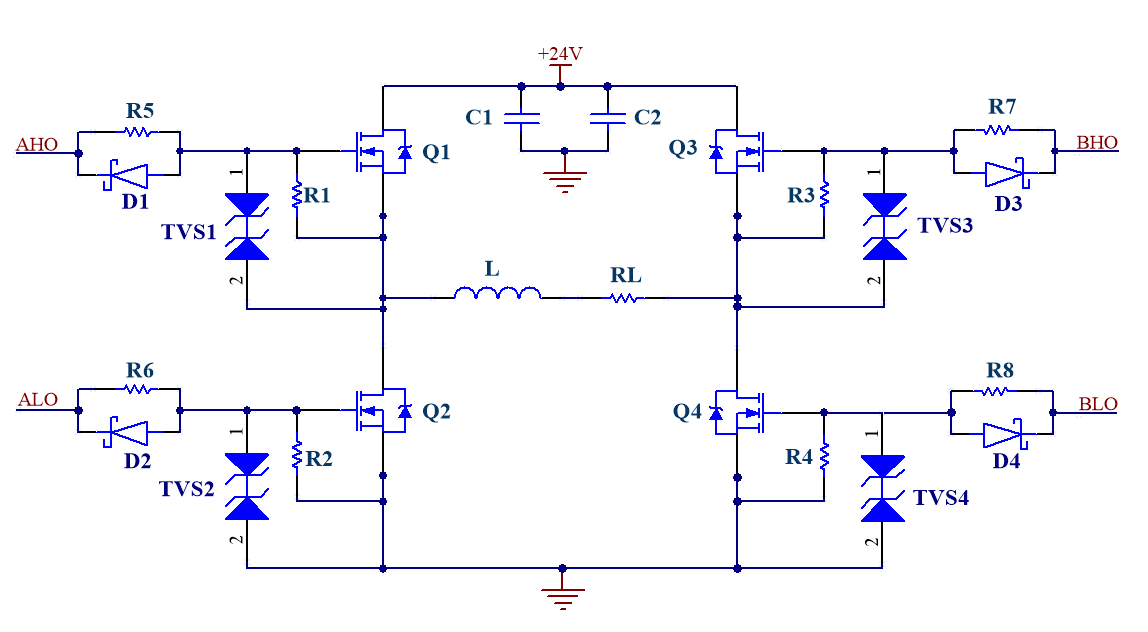
\includegraphics[scale=0.5]{puenteH-capacitores-fuente.png}
	\caption{Forma de onda de la corriente en $C_1$ y $C_2$.}
	\label{fig:img_puenteH-capacitores-fuente.png}
\end{figure}

\begin{figure}[H]
	\centering
	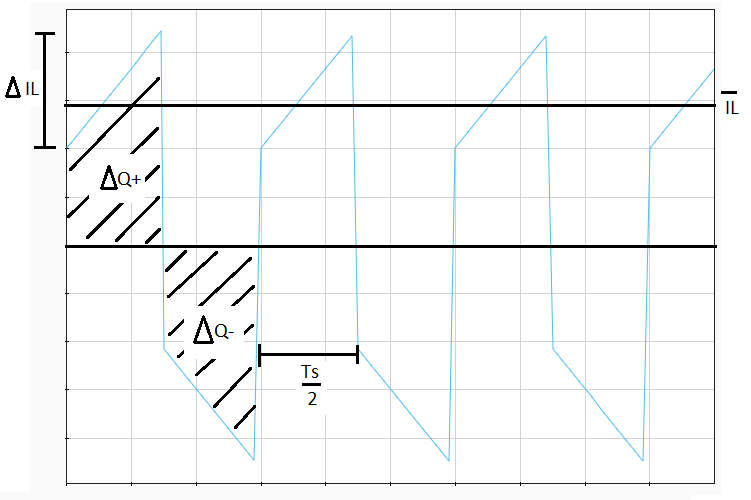
\includegraphics[scale=0.6]{Corriente-capacitores.png}
	\caption{Forma de onda de la corriente en $C_1$ y $C_2$.}
	\label{fig:img_ccorriente-capacitores}
\end{figure}

\noindent Por el electroimán circula una corriente media de aproximadamente $21\:A$ en condiciones normales de trabajo. Por lo tanto, la carga del capacitor se puede calcular como:

\begin{equation} 
	\begin{aligned}
		\Delta Q &= \int I dt\\	
	\end{aligned}
\end{equation}

\begin{equation} 
	\begin{aligned}
		\Delta Q ^+ &= \frac{T_S}{2}*\Delta I_L * \frac{1}{2} + (<I_L> -\frac{\Delta I_L}{2})*\frac{T_S}{2}\\
	\end{aligned}
\end{equation}

\begin{equation} 
	\begin{aligned}
		\Delta Q ^+ &= <I_L> *\frac{T_S}{2}\\
	\end{aligned}
\end{equation}

\noindent Con $\Delta I_L=500 \:mA$ y $T=0.47\:ms$ que corresponde a $Y_g = 2 \:mm$ según la tabla \ref{tab_mediciones}.

\begin{equation} 
	\Delta Q = 21\:A * \frac{0.47\:ms}{2} \approx 5\:mC
\end{equation}

\noindent Al considerar que un \textsl{ripple} de $\Delta V=500 \:mV$ es aceptable, se obtiene un valor de:

\begin{equation} 
	c = \frac{\Delta Q}{\Delta V} = 10 \:mF
\end{equation}

\noindent Dado que por los capacitores circula una corriente elevada ($21.25 A$) es recomendable disminuir la ESR total para minimizar la potencia disipada. Por lo tanto, se colocan capacitores en paralelo de baja ESR, como se muestra en la figura \ref{fig:img_capacitores-fuente}.

\begin{figure}[H]
	\centering
	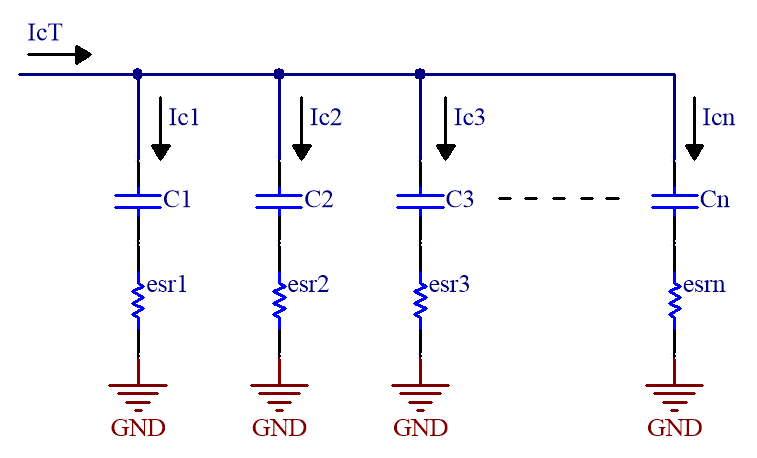
\includegraphics[scale=0.5]{Capacitores-fuente.png}
	\caption{Capacitores de la fuente.}
	\label{fig:img_capacitores-fuente}
\end{figure}


\begin{equation} 
	C = C1 + C2 + ... + C_n
\end{equation}


\noindent Si todos los valores de ESR son iguales se obtiene:

\begin{equation} 
	R_T = \frac{R_{ESR}}{n}
\end{equation}

\noindent Por lo tanto, se puede calcular la potencia que disipan como:

\begin{equation}\label{eq_potencia} 
	P = I^2 * R_T = 21.25^2 * \frac{R_{ESR}}{n}
\end{equation}

\noindent Se decidió utilizar 6 capacitores  EKY-350ELL222MM25S del fabricante Chemi-Con. Estos tienen una capacidad de $2200 \:uF$ con un rating de tensión de $50\:V$ y una ESR de $17 \:\Omega$ (datos obtenidos de \cite{EKY-350ELL222MM25S}) . De esta forma, al reemplazar en la ecuación \ref{eq_potencia} se obtiene que la potencia disipada es de: 

\begin{equation} 
	P=1.28\:W
\end{equation}

\subsection{Etapa de entrada y restador}

En esta sección se diseña la implementación circuital correspondiente a la etapa que realiza la resta entre la tensión de referencia, afectada por $K_{in}$, y la realimentación de la tensión proporcional a la corriente, como se muestra en el diagrama en bloques \ref{fig:img_diag-en-bloques-conH-y-Kin}.



En principio se calcula la ganancia de entrada $K_{in}$ utilizando la ecuación \ref{eq_kin} y teniendo en cuenta la ganancia del sensor de efecto Hall elegido:

\begin{equation}
	K_{in}=6\:\frac{A}{V}*53.33\:\frac{mV}{A}=0.32
\end{equation}

Se desea implementar un circuito que realice la operación matemática 

\begin{equation}\label{eq_Ve-circuito_1}
	V_e=K_{in}*V_{IL_{ref}} - V_{IL_{feed}}
\end{equation}

Para ello se utiliza un circuito basado en un amplificador operacional alimentado con una fuente simple de $5\:V$. Debido a que se usa una alimentación simple, es necesario polarizar su salida en un punto de operación $V_{op}=2.5\:V$ para permitir excursiones positivas y negativas de la señal. Por lo tanto la ecuación \ref{eq_Ve-circuito_1} se modifica agregando este punto de operación y se obtiene:

\begin{equation}\label{eq_Ve-circuito}
V_e=K_{in}*V_{IL_{ref}} - V_{IL_{feed}} + V_{op}
\end{equation}

En la figura \ref{fig:img_etapa-de-entrada} se muestra el circuito propuesto. 


\begin{figure}[H]
	\centering
	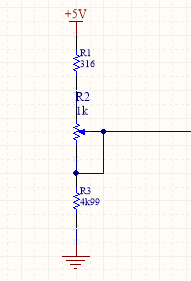
\includegraphics[scale=0.7]{Etapa-de-entrada.png}
	\caption{Etapa de entrada y restador.}
	\label{fig:img_etapa-de-entrada}
\end{figure}

Para determinar los valores de resistencia que se deben utilizar se realiza el análisis del circuito de la figura \ref{fig:img_etapa-de-entrada} y se obtiene la relación entre la salida $V_e$ y todas sus entradas:

\begin{equation*}
	V_e = \frac{R_{2}//R_{3}}{R_{1}+R_{2}//R_{3}}*\frac{R_{4}+R_{5}}{R_{5}}*V_{iLRef}-\frac{R_{4}}{R_{5}}*V_{iLF}+\frac{R_{1}//R_{3}}{R_{2}+R_{1}//R_{3}}*\frac{R_{4}+R_{5}}{R_{5}}* V_{op}
\end{equation*}

Por lo tanto, al igualarla con la expresión \ref{eq_Ve-circuito} resultan las siguientes ecuaciones de diseño:

\begin{equation} \label{eq_ve_operacional-1}
	\frac{R_{2}//R_{3}}{R_{1}+R_{2}//R_{3}}*\frac{R_{4}+R_{5}}{R_{5}} = K_{in} = 0.32
\end{equation}

\begin{equation} \label{eq_ve_operacional-2}
	\frac{R_{4}}{R_{5}} = 1
\end{equation}

\begin{equation} \label{eq_ve_operacional-3}
	\frac{R_{1}//R_{3}}{R_{2}+R_{1}//R_{3}}*\frac{R_{4}+R_{5}}{R_{5}} = 1
\end{equation}

De estas relaciones se obtiene que $R_{4}=R_{5}$. Luego al reemplazar en las ecuaciones \ref{eq_ve_operacional-1}, \ref{eq_ve_operacional-2} y \ref{eq_ve_operacional-3} resulta:

\begin{equation*}
	\frac{R_{2}//R_{3}}{R_{1}+R_{2}//R_{3}}= 0.16
\end{equation*}

\begin{equation*}
	\frac{R_{1}//R_{3}}{R_{2}+R_{1}//R_{3}}= 0.5
\end{equation*}

Tomando un valor de $R_{1} = R_{4} = 10\:k\Omega$ resulta en $R_{3}=4.7\:k\Omega$ y $R_{2}=3.2\:k\Omega$. Por lo tanto se obtiene a la salida del circuito la ecuación \ref{eq_ve_operacional}.

\begin{equation} \label{eq_ve_operacional}
	V_e = 0.32 * V_{IL_{ref}} - V_{IL_{feed}} + V_{op}
\end{equation}


\subsection{Adaptación de salida del sensor de corriente}

Para obtener la señal de realimentación ($V_{IL_{feed}}$) se debe adaptar la salida del sensor de efecto Hall a valores acordes a la señal de referencia. Esta última tiene valores de tensión entre $0\:V$ y $5\:V$ que se corresponden con una corriente entre $0\:A$ y $30\:A$. La salida del sensor ($V_{sns}$) está dada por:

\begin{equation}
	V_{sns}=I_L*H_0+V_{op}
\end{equation}

Esta tiene un punto de operación $V_{op}=2.5\:V$. Cuando la corriente es positiva, $V_{sns}$ estará por encima del punto de operación, mientras que para corriente negativa estará por debajo. Para que los valores de $V_{sns}$ coincidan con los de $V_{IL_{ref}}$ se le debe restar el punto de operación. Para ello se implementa un circuito restador basado en un amplificador operacional, que se muestra en la figura \ref{fig:img_resta-Vbias}.

\begin{figure}[H]
	\centering
	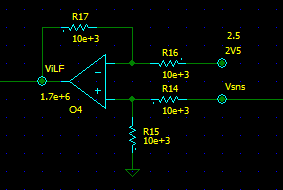
\includegraphics[scale=0.5]{Resta-Vbias.png}
	\caption{Resta de $V_{op}$ al sensor de efecto Hall.}
	\label{fig:img_resta-Vbias}
\end{figure}

Al utilizar este circuito se recortan los valores de $V_{sns}$ que se encuentren por debajo de $V_{op}$. Esto significa que se recortan los valores negativos de la corriente del electroimán.


La salida de este circuito queda determinada por:

\begin{equation}
	V_{IL_{feed}}=V_{sns}*\frac{R_{15}}{R_{14}+R_{15}}*\frac{R_{16}+R_{17}}{R_{16}}-V_{op}*\frac{R_{17}}{R_{16}}
\end{equation}

Como se desea que esta etapa sea un restador puro, se deben elegir valores para las resistencias que cumplan:

\begin{equation}
	\frac{R_{17}}{R_{16}}=1
\end{equation}

\begin{equation}
	\frac{R_{15}}{R_{14}+R_{15}}*\frac{R_{16}+R_{17}}{R_{16}}=1
\end{equation}

Estas ecuaciones se cumplen si todos los valores de resistencias son iguales. Es decir, $R_{14}=R_{15}=R_{16}=R_{17}$. Por lo tanto, se elige que estas resistencias sean de $10\:k\Omega$.

Finalmente, la salida de este circuito queda:

\begin{equation} \label{eq_salida_restador_hall}
	V_{IL_{feed}}=V_{sns}-V_{op}=I_L*H_0
\end{equation}

La ecuación \ref{eq_salida_restador_hall} es válida únicamente para $I_L>=0\:A$. Para valores de $I_L<0\:A$, la salida será $V_{IL_{feed}}=0$.

Si bien en el dispositivo levitador se desea que la corriente media del electroimán sea siempre positiva, este circuito tiene la desventaja de que elimina completamente cualquier corriente instantánea que sea negativa. Como se mencionó en la sección \ref{sec_topologia-fuente-alimentacion}, es necesario permitir una excursión de corriente negativa para el correcto funcionamiento del controlador, por lo tanto a continuación se propone una solución a este inconveniente.

\subsubsection{Ajuste para permitir corrientes negativas}

Debido a que el circuito encargado de realimentar la salida del sensor solo permite excursiones positivas de la corriente mientras que las negativas son recortadas, se presenta el problema de que si la corriente del electroimán se hace negativa instantáneamente, la tensión de salida del sensor de efecto Hall será menor a $V_{op}$. Por lo tanto, la salida del operacional será recortada y el sistema quedará a lazo abierto. Para solucionar este problema se analizaron dos alternativas:

\begin{itemize} 
	\item Elevar el \textsl{set-point}  $V_{op}$ del sensor de efecto Hall.
	
	\item Utilizar una alimentación bipolar para el operacional de realimentación.
\end{itemize}

Entre estas se eligió la primera alternativa, ya que se puede implementar con mayor facilidad en el circuito. Hay que tener en cuenta que, al incrementar el \textsl{offset} del sensor, también se debe incrementar en la misma proporción la tensión de referencia de la etapa de entrada al controlador de corriente ($V_{op}$ en figura \ref{fig:img_etapa-de-entrada}), pero para el resto de los circuitos la tensión $V_{op}$ sigue manteniendo su valor de $2.5\:V$.

A continuación se debe determinar qué valor utilizar para la tensión de referencia del sensor de efecto Hall y de la etapa de entrada. Para ello se debe calcular el mínimo de tensión que podría entregar el sensor de efecto Hall. Esto se da cuando la referencia del controlador de corriente es de $0\:V$, con lo que la corriente media del electroimán es $0 \:A$ con una excursión de $±250\:mA$. Esto significa una tensión de salida del sensor de efecto Hall de $13.3\:mV$ por encima y debajo del \textsl{offset}. Para tomar un margen se incrementa a $V_{op}=2.6\:V$. 

Teniendo en cuenta este cambio en el punto de operación, la salida de la etapa de acondicionamiento para la salida del sensor de efecto Hall queda:

\begin{equation} \label{eq_salida_restador_hall_2}
	V_{IL_{feed}}=V_{sns}-2.5V =I_L*H_0 + 2.6V - 2.5V =I_L*H_0+0.1V
\end{equation}

Por otro lado, al considerar el cambio en el punto de operación, es necesario volver acalcular algunos valores de resistencias de la etapa de entrada de las ecuaciones \ref{eq_ve_operacional-1} y \ref{eq_ve_operacional-3}.


A continuación se muestran los circuitos correspondientes a la etapa de entrada y acondicionamiento de salida del sensor, con la modificación en el punto de operación:

\begin{figure}[H]
	\centering
	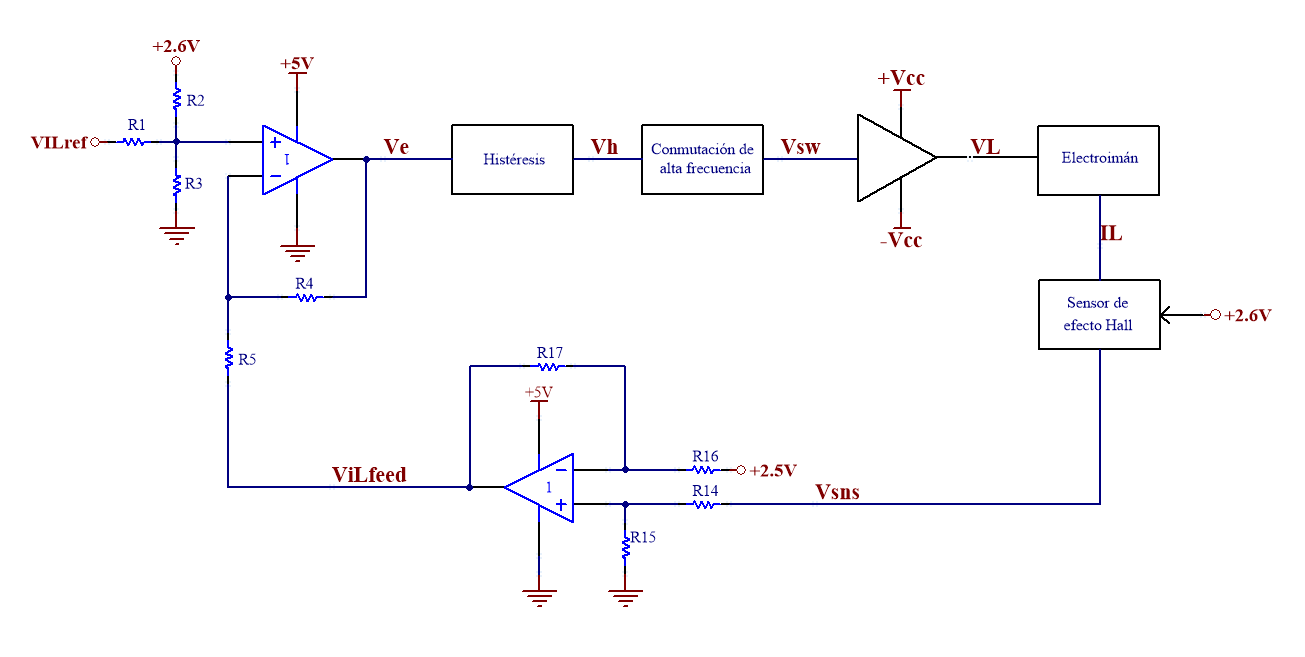
\includegraphics[scale=0.5]{circuito-de-entrada-completo.png}
	\caption{Circuitos de etapa de entrada completo.}
	\label{fig:img_circuito-de-entrada-completo.png}
\end{figure}

\colorbox{red}{Agregar 2.6 a R2 y a sensor de efecto hall y 2.5 a R16 y agregar el operacional para la conmutacion como en el diagrama}

\subsection{Comparador con histéresis y oscilador auxiliar}

En esta sección se analiza la implementación circuital de la etapa de conmutación, compuesta por un comparador con histéresis y un oscilador auxiliar.

\subsubsection{Circuito del oscilador auxiliar}

Como se mencionó en la sección \ref{sec_cap_bootstrap} es necesario agregar una etapa de oscilación auxiliar para permitir la carga de los capacitores de bootstrap en un intervalo de tiempo regular.

Para implementar el oscilador de alta frecuencia se propone la topología circuital mostrada en la figura \ref{fig:img_frecuencia-auxiliar}. Esta genera una señal pulsada con ciclo de trabajo 90\% en su salida a partir de el valor de la tensión $V_h$ en su entrada con el agregado de una inversión de fase. 

\begin{figure}[H]
	\centering
	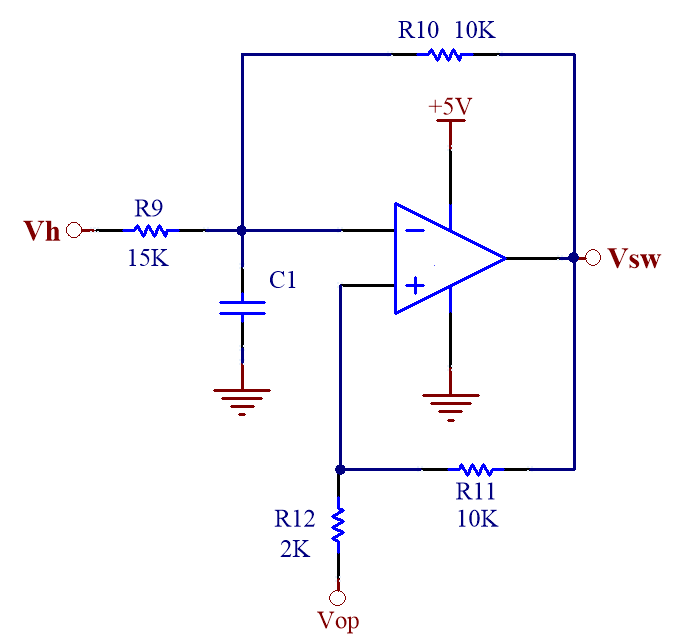
\includegraphics[scale=0.7]{conmutacion-auxiliar.png}
	\caption{Circuito oscilador de frecuencia auxiliar.}
	\label{fig:img_frecuencia-auxiliar}
\end{figure}

Pueden darse dos casos:

1- $V_h=5\:V$ entonces la salida estará 90\% del tiempo en $0\:V$ y  el resto en $5\:V$. 

2- $V_h=0\:V$ entonces la salida estará 90\% del tiempo en $5\:V$ y el resto en $0\:V$.

\colorbox{red}{hacer calculo de componentes}

Este circuito es un oscilador de onda pulsada basado en un comparador con histéresis con el agregado de una red de realimentación negativa RC. Sus ecuaciones de diseño son:

\colorbox{red}{capaz podemos poner directamente unas ecuaciones de diseño en vez de analizar todo el comportamiento del circuito}

%Para generar esta conmutación se agrega el oscilador que se observa en la figura \ref{fig:img_frecuencia-auxiliar} a la salida del comparador con histéresis. La frecuencia de conmutación se puede obtener en función de $C_1$ como:
%
%\begin{equation} 
%	F_{aux} = \frac{4.5*10^{-5}}{C1} [Hz]
%\end{equation}



\colorbox{red}{A la imagen de abajo no la saqué todavia para ver los valores de los componentes}
\begin{figure}[H]
	\centering
	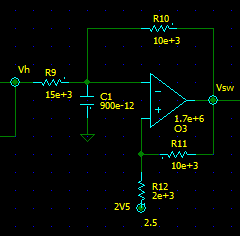
\includegraphics[scale=1]{Frecuencia-auxiliar.png}
	\caption{Circuito oscilador de frecuencia auxiliar.}
	\label{fig:img_frecuencia-auxiliarasdas}
\end{figure}

\subsubsection{Circuito del comparador con histéresis}

Para implementar el comparador con histéresis se utiliza un amplificador operacional realimentado positivamente. Para el diseño del comparador se tiene en cuenta la inversión de signo que aporta la etapa de oscilador de alta frecuencia para cancelarla. Debido a que se definió que la corriente de salida del electroimán tenga un \textsl{ripple} de $500\:mA$, al afectarla por la ganancia del sensor de corriente ($H_0$) se obtiene un ancho de histéresis de $26.665\:mV$. El circuito implementado se muestra en la figura \ref{fig:img_comp-con-hist}.

\begin{figure}[H]
	\centering
	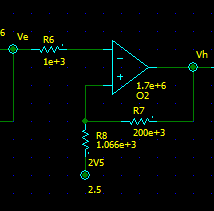
\includegraphics[scale=1]{Comparador-con-histeresis.png}
	\caption{Comparador con histéresis.}
	\label{fig:img_comp-con-hist}
\end{figure}

El funcionamiento de este circuito depende de la tensión de entrada $V_e$ y la tensión en la entrada no inversora del operacional $V^+$ y esta, a su vez, depende de la tensión de salida $V_h$. El circuito tiene dos estados posibles:

1- Cuando $V_e<V^+$ la salida será $V_h=5V$

2- Cuando $V_e>V^+$ la salida será $V_h=0V$

Para obtener una expresión para la salida en función de la entrada, primero es necesario conocer el valor de $V^+$.
Las ecuaciones son las siguientes:

\begin{equation} 
	V^+ = V_h*\frac{R_{8}}{R_{8}+R_{7}} + 2.5V*\frac{R_{7}}{R_{8}+R_{7}}
\end{equation} 

La tensión diferencial entre las patas $V^+$ y $V^-$ es $Vd=(V^+)-(V^-)$. Por lo tanto se pueden plantear dos casos: 

1- Cuando $V_e>V^+$ entonces $V_h=0V$. Por lo tanto:

\begin{equation}
	V^+_{off}=2.5*\frac{R_{7}}{R_{8}+R_{7}}
\end{equation}

2- Cuando $V_e<V^+$ entonces $V_h=5V$. Resulta:

\begin{equation}
	V^+_{on}=2.5*\frac{R_{7}}{R_{8}+R_{7}} + 5V*\frac{R_{8}}{R_{8}+R_{7}}=V^+_{off}+5V*\frac{R_{8}}{R_{8}+R_{7}}
\end{equation}

Como $V_{e}$ tiene forma triangular, inicialmente se tendrá una forma de onda de rampa creciente tal que $V_e < V^+_{on}$. Por lo tanto, la salida del comparador será $V_{h}=5\:V$. Luego, cuando $V_e > V^+_{off}$ se alternará la salida del comparador a $V_{h}=0\:V$ alternando la señal a una rampa decreciente hasta que nuevamente se alcance $V_e<V^+$. Este ciclo de histéresis se mantiene constante.

Para obtener un ancho de histéresis de $26,665 mV$ entonces la diferencia entre el punto mas alto y mas bajo debe ser:

\begin{equation}
	V^+_{on}-V^+_{off} = 5V*\frac{R_{8}}{R_{8}+R_{7}}= 26,665 mV
\end{equation}

Si se toma $R_{7}=200 \:k\Omega$ se obtiene $R_{8}=1072 \;\Omega$ por lo tanto se toma un valor comercial de $R_{8}=1066\:\Omega$. De esta forma se obtiene el ancho de histéresis deseado.

\subsection{Elección de amplificadores operacionales}

Para implementar los circuitos planteados en las secciones anteriores se decidió utilizar el amplificador operacional MCP664 \colorbox{red}{Agregar datasheet} ya que pueden ser alimentados mediante una fuente de tensión simple de $5\:V$ y admiten a su salida una excursión de tensión completa entre $0\:V$ y $5\:V$. 

\subsection{Conexión de oscilador con HIP???}
El HIP tiene 4 señales de control, cada una encargada de controlar una llave. Sin embargo, como se mencionó en la sección \ref{sec_topologia-fuente-alimentacion}, con una señal de control es suficiente para manejar el puente H ya que dos de ellas son iguales y las otras dos están invertidas con respecto a las primeras. Esta señal de control es la salida del oscilador de alta frecuencia. Por lo tanto, conexionado resultante se muestra en el circuito de la figura daddasdasADSDAS.

\colorbox{red}{poner diagrama de conexión, señales de control HIP con oscilador}


\section{SIMULACIONES??}

Se utilizó el software de simulación de circuitos electrónicos NL5 para construir una representación circuital del controlador de corriente y comprobar el correcto funcionamiento del circuito según los parámetros con los que se diseñó. El circuito armado se muestra en la figura \ref{fig:circuito_simulacion_final}.


\begin{figure}[H]
	\centering
	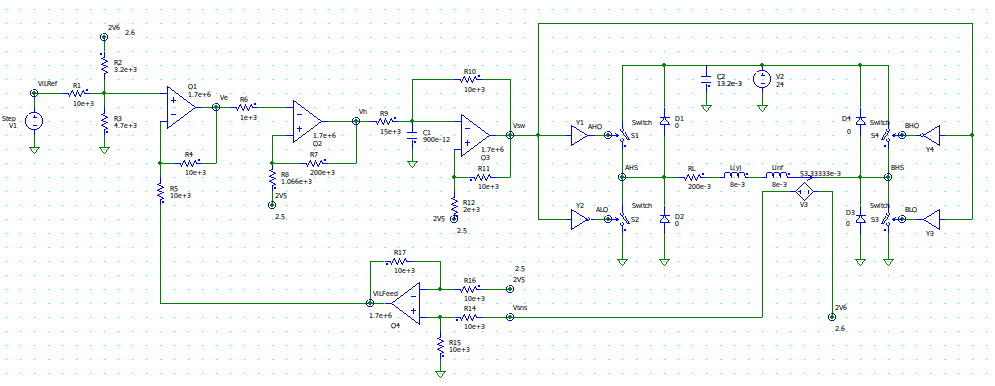
\includegraphics[width=1\linewidth]{circuito_simulacion_final.png}
	\caption[Circuito armado para la simulación]{}
	\label{fig:circuito_simulacion_final}
\end{figure}


\subsection{Señales en régimen permanente}

En las figuras \ref{fig:simulacion_regimen_permanente_1} y \ref{fig:simulacion_regimen_permanente_2} se muestran algunas señales de intéres del controlador de corriente funcionando en régimen permanente con una tensión de referencia $V_{IL_{ref}}=1\:V$ y el valor de inductancia correspondiente a $Y_g=4\:mm$.

\begin{figure}[H]
	\centering
	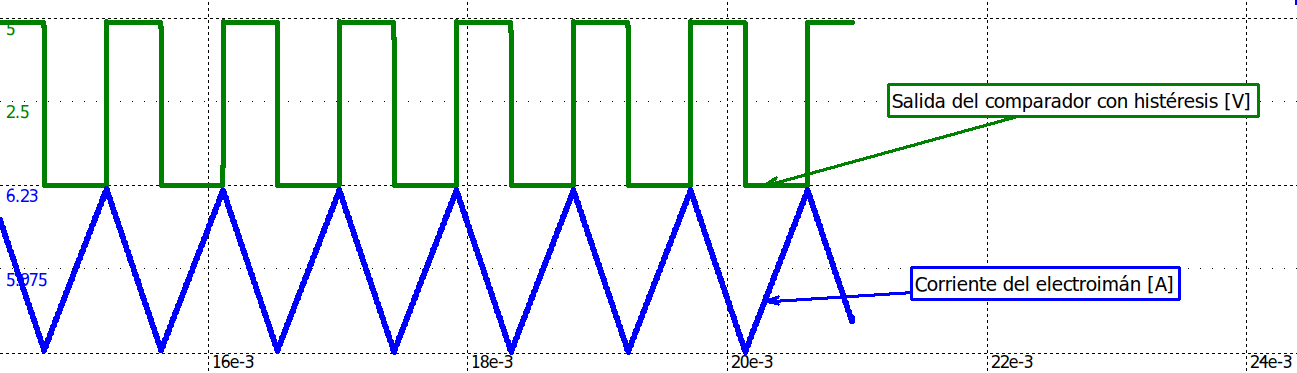
\includegraphics[width=1\linewidth]{simulacion_regimen_permanente_1.png}
	\caption{Simulación de señales en régimen permanente.}
	\label{fig:simulacion_regimen_permanente_1}
\end{figure}

\begin{figure}[H]
	\centering
	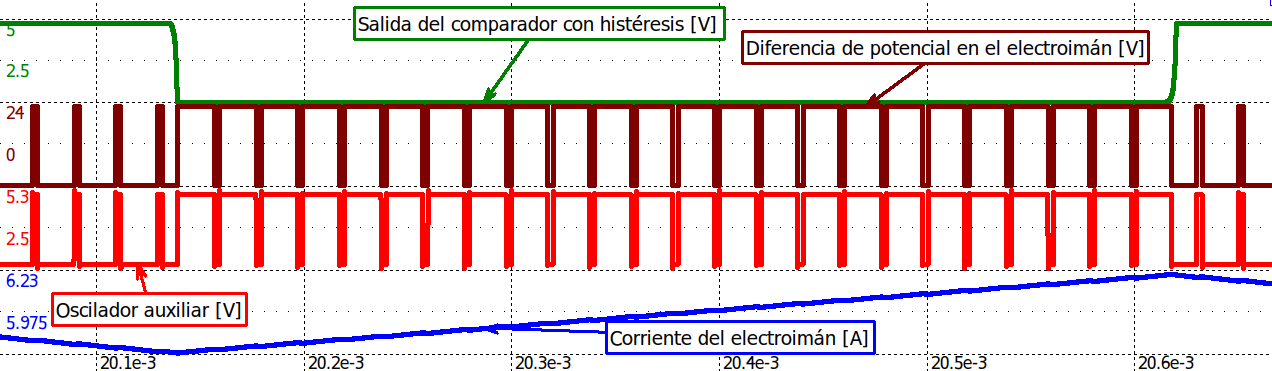
\includegraphics[width=1\linewidth]{simulacion_regimen_permanente_2.png}
	\caption{Simulación de señales de alta frecuencia en régimen permanente.}
	\label{fig:simulacion_regimen_permanente_2}
\end{figure}


De esta simulación se pueden realizar mediciones sobre variables del sistema y comprobar si coinciden con los parámetros que se utilizaron para el diseño. Para las mediciones se utilizó la funcionalidad de cursores que tiene el programa NL5 y se agruparon los resultados en la tabla \ref{tab_mediciones_simulacion}

%Se midió:
%VLon = +24V
%VLoff = -24V
%Fsw = 49.8 kHz %de vl
%Ilmed = 5.97A
%deltaIL = 509mA
%freq = 1.08 kHz %de baja frecuencia
%Ton = 17.57us
%Toff = 2.5us
%Ttotal = 20.06
%d = 87\%

\begin{table}[H]
	\begin{center}
		\begin{tabular}{| c | c | c |}
			\hline
			Variable & Resultado medido & Resultado teórico \\ \hline
			$\overline{I_L}$ [A] & $5.97$ & $6$ \\ \hline
			$\Delta I_L$ [mA] & 509 & 500 \\ \hline
			$F_{planta}$ [Hz]& 1080 &	1000 \\ \hline
			$V_{L_{on}$ [V]&	24 & 24 \\ \hline
			$V_{L_{off}}$ [V]& -24 & -24 \\ \hline
			$F_{aux}$ [kHz] & 49.8 & 50 \\ \hline
			$d$ [\%] & 87 & 90 \\ \hline
		\end{tabular}
		\caption{Valores calculados y medidos en función del entrehierro.}
		\label{tab_mediciones_simulacion}
	\end{center}
\end{table}

\colorbox{red}{ver si modificamos los nombres mas arriba como Fplanta, Faux, etc...}

\begin{figure}[H]
	\centering
	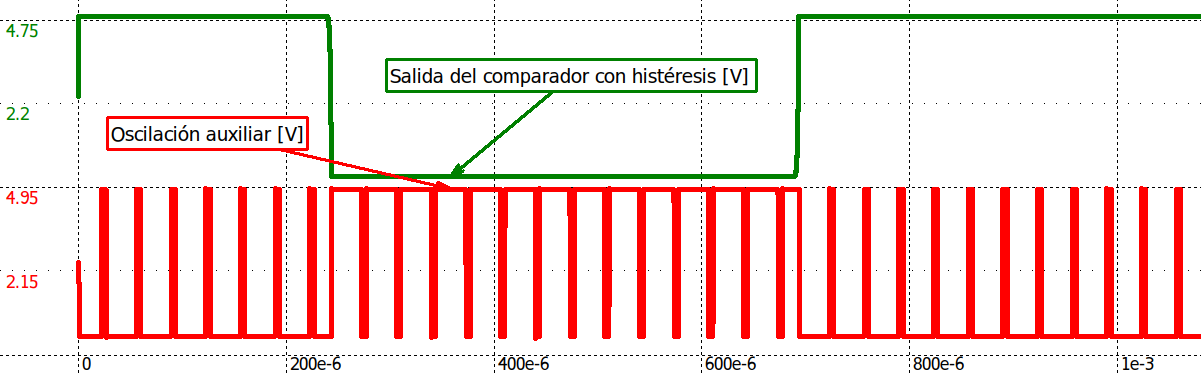
\includegraphics[width=1\linewidth]{simulacion_auxiliar.png}
	\caption{Simulación de conmutación auxiliar.}
	\label{fig:simulacion_auxiliar}
\end{figure}

\begin{figure}[H]
	\centering
	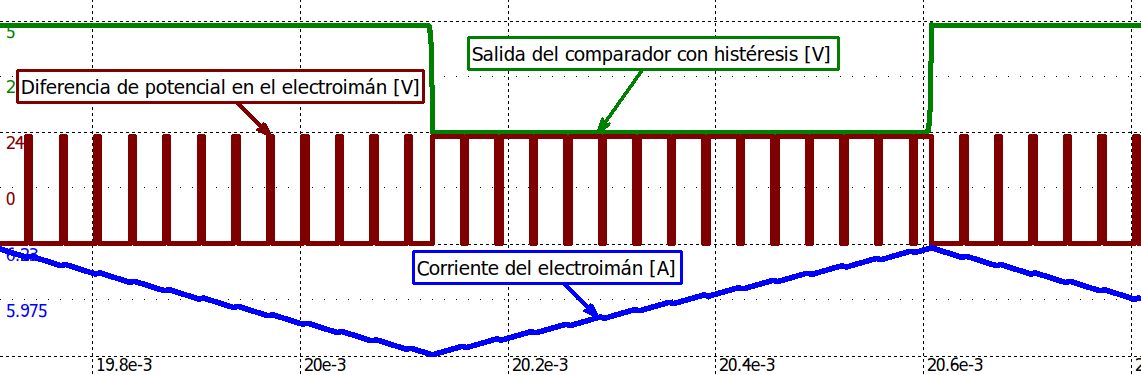
\includegraphics[width=1\linewidth]{simulacion_alimentacion.png}
	\caption{Simulación de tensión de alimentación en el electroimán.}
	\label{fig:simulacion_alimentacion}
\end{figure}

\subsection{Simulación de escalón en la referencia de corriente}

En la figura \ref{fig:simulacion_escalon} se muestra como reacciona el sistema ante un cambio en la tensión de referencia de corriente. El sistema comienza estable en un valor de corriente media $I_L=0\:A$ y luego del cambio de referencia se estabiliza en $I_L=6\:A$.

\begin{figure}[H]
	\centering
	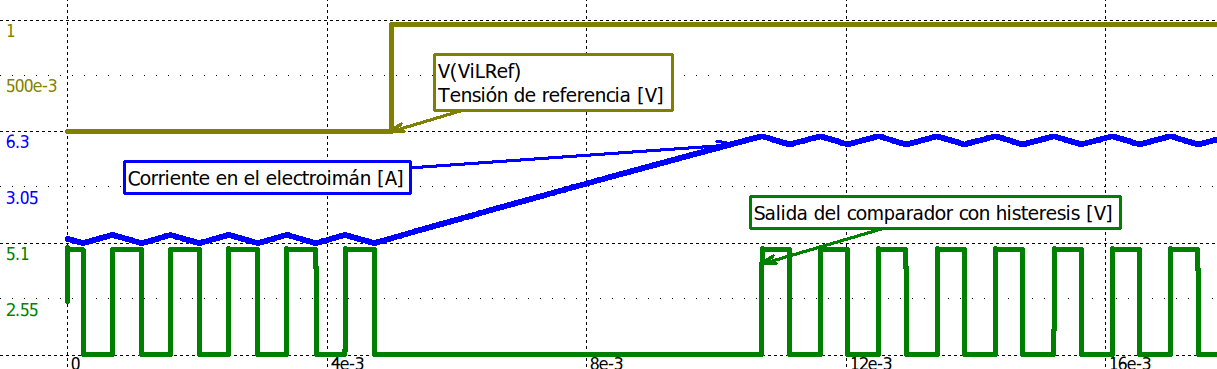
\includegraphics[width=1\linewidth]{simulacion_escalon.png}
	\caption{Simulación de escalón en la referencia de corriente.}
	\label{fig:simulacion_escalon}
\end{figure}

\section{Características estáticas y dinámicas del controlador}

Si bien el controlador de corriente está basado en un control de tipo no lineal, es posible obtener sus características estáticas y dinámicas para luego utilizarlas en el diseño del sistema de control de levitación.

\subsection{Corriente media del electroimán}

\noindent Para saber la corriente media que hay a la salida al aplicarle cierta tensión en la entrada, se utiliza la transferencia de lazo cerrado (sin considerar polos, y suponiendo alta ganancia de lazo abierto):

\begin{equation} 
I_L = V_{IL_{ref}} * \frac{K_{in}}{H_0} = V_{IL_{ref}} * 6\:\frac{A}{V}
\end{equation}

\subsection{Frecuencia de conmutación de la corriente}

\noindent La frecuencia de conmutación del sistema se obtiene con:

\begin{equation}\label{eq_frec-sw} 
F_{SW} = \frac{V_{cc}}{2*\Delta I_L * L(Y_g)}
\end{equation}

\noindent Para $Y_g = 4 \:mm $ se tiene una inductancia $L(4\:mm) = 16.44 \:mHy$ , lo cual resulta en una frecuencia $F_{SW }= 1460 \:Hz$ .

\subsection{Ancho de banda del controlador}\label{esccion_AB_Controlador} 

\noindent La dinámica del controlador, al depender de la inductancia, lo hace también del entrehierro. El ancho de banda (o velocidad con que responde) está limitado por la constante de tiempo del inductor con su resistencia serie. Juntas forman un sistema lineal de primer orden, con un polo en: 

\begin{equation} \label{eq_frec-angular}
\omega _{polo} = \frac{R_L}{L(Y_g)}
\end{equation}

\noindent Al tomar las condiciones del problema en el punto de linealización con $Y_{0}=4\:mm$, resulta una inductancia $L = 7.55 \:mHy + 8.89 \:mHy$. Luego, al considerar la resistencia del bobinado $R_L=0.2\:\Omega$, se calcula la ubicación del polo:

\begin{equation} 
\omega _{polo} = \frac{0.2\:\Omega}{16.44 \:mHy} = 12.17 \:rad/s
\end{equation}

\noindent La tabla \ref{tab_mediciones} muestra  entre qué valores de frecuencia se ve afectada la forma de onda al modificarse la distancia de separación.

\begin{equation} \label{eq_DeltaT}
\Delta T [s] = \frac{\Delta I_L * (L(Y_g) + L_{\infty})}{V_{BUS}}
\end{equation}

\noindent En la ecuación \ref{eq_DeltaT}, $\Delta T$ representa el tiempo de crecimiento o de decrecimiento de la rampa de corriente (sin considerar la resistencia del bobinado) en torno al valor nominal. El doble de este tiempo es igual al periodo de la corriente triangular $(2*T=\frac{1}{F_{SW}})$.

\noindent Según las mediciones de inductancia realizadas y, al aplicar las ecuaciones \ref{eq_frec-sw}, \ref{eq_frec-angular} y \ref{eq_DeltaT}, se obtuvo la tabla \ref{tab_mediciones}.


\begin{table}[H]
	\begin{center}
		\begin{tabular}{| c | c | c | c | c |}
			\hline
			$Y_g\:[mm]$ & $L(Y_g)\:[mHy]$ & $\Delta T\:[ms]$ & $F_{SW}\:[Hz]$ & $\omega _{polo}\:[rad/s]$\\ \hline
			0 & 76.45 & 1.59 & 313.93 & 2.62\\ \hline
			1 & 33.42 & 0.70 & 718.13 & 5.98\\ \hline
			2 & 22.64 &	0.47 & 1060.07 & 8.83\\ \hline
			3 &	18.8 & 0.39 & 1276.60 & 10.64\\ \hline
			4.4 & 15.5 & 0.32 & 1548.39 & 12.90\\ \hline
			5.2 & 14.7 & 0.31 & 1632.65 & 13.61\\ \hline
			6.5 & 14.4 & 0.30 & 1666.67 & 13.89\\ \hline
			8.23 & 12.4 & 0.26 & 1935.48 & 16.13\\ \hline
			$\infty$ & 8.89 & 0.19 & 2699.66 & 22.5	\\ \hline
		\end{tabular}
		\caption{Valores calculados y medidos en función del entrehierro.}
		\label{tab_mediciones}
	\end{center}
\end{table}

\subsection{Transferencia lineal del controlador de corriente}

\noindent En la ecuación \ref{eq_TLC-cc} se muestra la transferencia linealizada del controlador de corriente para una distancia de separación de $Y_g=4\:mm$. Esta será luego utilizada para realizar el diseño de las etapas de compensación del levitador completo. Si bien la dinámica del controlador corriente se ve afectada por la distancia de separación, para el diseño de la compensación se tendrá en cuenta únicamente la dinámica para $Y_g=4\:mm$.

\begin{equation} \label{eq_TLC-cc}
G_{iL}(s) = \frac{6}{1+\frac{s}{12.17}}
\end{equation}
